
% Main tex file for Alex Ledger's thesis

\documentclass[12pt,twoside]{reedthesis}
\usepackage{graphicx,latexsym} 
\usepackage{amssymb,amsthm,amsmath}
\usepackage{longtable,booktabs,setspace} 
\usepackage[hyphens]{url}
\usepackage{rotating}
\usepackage{natbib}
\usepackage{hhline}
\usepackage{multirow}
\usepackage{adjustbox}
\usepackage{algorithm,algpseudocode}
\usepackage{changepage}
\usepackage{circuitikz}
\usepackage{protocolj}


% Alex L's macros 
% taken and co-opted from a variety of sources

% generic commands
\newcommand{\NN}{\mathbb{N}}
\newcommand{\RR}{\mathbb{R}}
\newcommand{\compindist}{\approx_C}

% definition counter
\newcounter{defcounter}
\setcounter{defcounter}{0}
\newenvironment{definition}{\medskip\noindent\refstepcounter{defcounter}{\bf Definition \thedefcounter}\hspace*{2pt}}{\hspace*{\fill}\nopagebreak[4]$\diamondsuit$\medskip}  

% block quote
\newenvironment{blockquote}{%
  \par%
  \medskip
  \leftskip=4em\rightskip=2em%
  \noindent\ignorespaces}{%
  \par\medskip}

% Author Macros -- colors: red, magenta, blue, orange
\newcounter{al}
\newcommand{\al}[1]{\textcolor{blue}{\{AL-\arabic{al}: #1\}}\addtocounter{al}{1}}
\newcounter{cat}
\newcommand{\cat}[1]{\textcolor{magenta}{\{CAT-\arabic{cat}: #1\}}\addtocounter{cat}{1}}
\newcommand{\ignore}[1]{}

% From CompGC paper
%\renewcommand{\sim}{S}
\newcommand{\Input}{\ensuremath{\textsf{Input}}\xspace}
\newcommand{\Output}{\ensuremath{\textsf{Output}}\xspace}
\newcommand{\Inputs}{\ensuremath{\textsf{Inputs}}\xspace}
\newcommand{\Outputs}{\ensuremath{\textsf{Outputs}}\xspace}
\newcommand{\SFOutputs}{{\sf {Outputs}}}
\newcommand{\Components}{\ensuremath{\textsf{Components}}\xspace}
\newcommand{\samples}{\gets} 

\newcommand{\Gates}{\text{Gates}}
\newcommand{\C}{\sf {C}}
\newcommand{\GC}{\sf {GC}}
\newcommand{\AllInputLabels}{\sf {AllInputLabels}}
\newcommand{\InputLabels}{\sf {InputLabels}}
\newcommand{\InputWires}{\text{InputWires}}
\newcommand{\OutputWires}{\text{OutputWires}}
\newcommand{\Wires}{\text{Wires}}
\newcommand{\A}{\mathcal{A}}
\newcommand{\OT}{\textsf{OT}} % or mathsf
\newcommand{\Enc}{\textsf{Enc}} % or mathsf
\newcommand{\Dec}{\textsf{Dec}}
\newcommand{\Gen}{\textsf{Gen}}
\newcommand{\EncInv}{\Enc^{-1}}
\newcommand{\EncDKC}{\textsf{EncDKC}}
\newcommand{\DecDKC}{\textsf{DecDKC}}
\newcommand{\EncDKCInv}{\EncDKC^{-1}}
\newcommand{\compIndist}{\approx_D}
\newcommand{\outputrv}{{\sf output}}
\newcommand{\viewrv}{{\sf view}}
\newcommand{\Ours}{\CompGC}
\newcommand{\CompGC}{\textsf{CompGC}\xspace}
\newcommand{\JustGarble}{\textsf{JustGarble}\xspace}
\newcommand{\LibGarble}{\textsf{LibGarble}\xspace}
\newcommand{\Naive}{\textsf{Naive}\xspace}
\newcommand{\scmc}{SCMC\xspace} % Single Communication Multiple Connnection

\newcommand{\Garble}{\sf{Garble}\xspace} 
\newcommand{\Link}{\sf{Link}\xspace} 
\newcommand{\Eval}{\sf{Eval}\xspace} 


\usepackage{hyperref}
\hypersetup{
    colorlinks=true,
    linkcolor=blue,
    filecolor=magenta,      
    urlcolor=cyan,
}

% Comment out the natbib line above and uncomment the following two lines to use the new 
% biblatex-chicago style, for Chicago A. Also make some changes at the end where the 
% bibliography is included. 
%\usepackage{biblatex-chicago}
%\bibliography{thesis}

\title{Implementing Improvements for Secure Function Evaluation}
\author{Alex Ledger}
\date{May 2016}
\division{Mathematics and Natural Sciences}
\advisor{Adam Groce}
\department{Mathematics}
\setlength{\parskip}{0pt}

\begin{document}

\maketitle
\frontmatter % this stuff will be roman-numbered
\pagestyle{empty} % this removes page numbers from the frontmatter

\chapter*{Acknowledgements}
I want to thank a few people.

% The preface is optional
% To remove it, comment it out or delete it.
\chapter*{Preface}
This is an example of a thesis setup to use the reed thesis document class.

\chapter*{List of Abbreviations}
You can always change the way your abbreviations are formatted. Play around with it yourself, use tables, or come to CUS if you'd like to change the way it looks. You can also completely remove this chapter if you have no need for a list of abbreviations. Here is an example of what this could look like:

\begin{table}[h]
\centering % You could remove this to move table to the left
\al{Do I need this?}
\begin{tabular}{ll}
	\textbf{ABC}  	&  American Broadcasting Company \\
	\textbf{CBS}  	&  Columbia Broadcasting System\\
	\textbf{CDC}  	&  Center for Disease Control \\
	\textbf{CIA}  	&  Central Intelligence Agency\\
	\textbf{CLBR} 	&  Center for Life Beyond Reed\\
	\textbf{CUS}  	&  Computer User Services\\
	\textbf{FBI}  	&  Federal Bureau of Investigation\\
	\textbf{NBC}  	&  National Broadcasting Corporation\\
\end{tabular}
\end{table}
	
\tableofcontents
\listoftables
\listoffigures

%!TEX root = thesis.tex

\chapter*{Abstract}

Secure computation is a cryptographic method for securely computing a function between two parties while preserving the privacy of the parties' inputs.
Some modern research into secure computation uses an offline/online scheme, where parties pre-process and exchange information in an offline phase prior to computing the function in an online phase. 
The offline/online setting has many advantages, namely that the online computation is very fast, but the setting is limiting, as the function that is being computed must be determined ahead of time.

This thesis is part of a larger project that created component-based garbled circuits to address some of the problems with the offline/online setting.
Component-based garbled circuits observe that many real-world functions are composed of standard components such as arithmetic operations, matrix operations and other common operations.
Component-based garbled circuits exchange many small, generic garbled components in an offline phase. 
Later in an online phase, the parties choose a function they wish to compute, and they stitch together the garbled components in order to create the function.

This thesis contributes two items to the larger project of component-based garbled circuits.
The first item is \textit{Single Communication Multiple Connections} (SCMC); SCMC is a technique that improves the online bandwidth of component-based garbled circuits.
The second item is an implementation, \CompGC, of component-based garbled circuits.
\CompGC is designed to be fast and secure; we run performance measurements on \CompGC, and we find that component-based garbled circuits offer considerable savings in online time and online bandwidth over other implementations of garbled circuits. 

\chapter*{Dedication}
You can have a dedication here if you wish.

	
\mainmatter % here the regular arabic numbering starts
\pagestyle{fancyplain} % turns page numbering back on

%!TEX root = thesis.tex


%The \introduction command is provided as a convenience.
%if you want special chapter formatting, you'll probably want to avoid using it altogether
\chapter*{Introduction}
     \addcontentsline{toc}{chapter}{Introduction}
\chaptermark{Introduction}
\markboth{Introduction}{Introduction}

Suppose that millionaires Alice and Bob wish to determine who is wealthier, but they do not want to disclose their wealth to each other.
Alice and Bob could tell a trusted third party their wealth, and then that trusted third party could tell Alice and Bob who is wealthier.
However, that method has many disadvantages, one being that they need to trust a third party.
What if there were a method that allows Alice and Bob to determine who is wealthier by only sending messages between themselves?

This classic problem is known as the \textit{millionaire problem}, and it is a special case of \textit{secure computation}.
Secure computation gives multiple parties the ability to jointly to compute an arbitrary function, while keeping each party's input private from all other parties.
In the millionaire problem, there are two parties, Alice and Bob, and they wish to compute the less than function.

We generalize secure computation to allow for an arbitrary number of parties to compute an arbitrary function amongst themselves. 
By generalizing secure computation, we open up many possible uses where secure computation can improve an existing process or allow for computations that are otherwise impossible or illegal. 
For example, we can run an election without a centralized body; we can perform an auction without using an auctioneer; and we can enable multiple hospitals with sensitive healthcare data to work together without sacrificing the privacy of their data.
While secure computation works with arbitrarily many parties, this thesis focuses on the special case where there are two parties, called two-party computation (2PC).

The most common method for performing 2PC is \textit{garbled circuits}.
In a garbled circuit protocol, the parties transform their function $f$ into a circuit. 
They then \textit{garble} their circuit, such that with a bit more information they can \textit{evaluate} the garbled circuit, recovering the answer to their function.
Garbling the circuit involves obscuring the truth value of each wire inside the circuit.
Once the truth values are obscured, the parties cannot learn any information as they process, or evaluate, the circuit: they only learn the answer to their function.

Garbled circuits have been heavily researched and optimized since their creation in the late 1980s.
For most of that period, garbled circuit protocols were too slow and cumbersome for usage in the real world, but as of late, the protocols have achieved speeds comparable to that of loading a webpage. 

In order to further increase the speed of garbled circuits, researchers split the garbled circuit protocol into two phases, an offline phase and an online phase.
In the offline phase, before the two parties determine their inputs to the function, the parties exchange as much information as feasible. 
later, when the parties decide to compute the function, and they determine determine their inputs to the function, the parties engage in an online phase, where they exchange more information and finish the garbled circuit protocol, whereby they recover the output to their function.
Using an offline/online protocol greatly reduces the latency of the computation - the time that it takes to go from determining inputs to acquiring an answer.

The offline/online system, while offering a number of benefits, is also limiting in that the function is determined ahead of time in the offline phase.
Say that millionaires Alice and Bob originally agree to find out who is wealthier, so they exchange information for that function ahead of time in the offline phase, but then at the beginning of the online phase, Alice and Bob change their minds. 
Instead, they now wish to verify that they are indeed both millionaires, and verify that the other party is not going bankrupt.
Since they exchanged information specific to the ``who is wealthier'' function during the offline phase, they are stuck. 
They cannot pivot and compute the new function without large computational sacrifices.

This thesis presents a new method called \textit{component-based} garbled circuits to solve this problem.
In the offline phase, instead of exchanging information corresponding to a single function, Alice and Bob exchange smaller pieces of information that can be stitched together to compute a class of functions.
For example, instead of exchanging a garbled circuit that computes the ``who is wealthier'' function, Alice and Bob exchange many garbled circuits which are \textit{components} or subparts of the less than function and other similar functions.
Then, during the online phase, Alice and Bob select the function that they wish to compute from the class of available functions, and build their function by \textit{chaining} pre-exchanged components.
With component-based garbled circuits, Alice and Bob have more flexibility. 
They are no longer stuck using their original function - they can securely compute a host of functions at their whim. 

This thesis is part of a larger project which created component-based garbled circuits; specifically, it contributes two items to the project.
The first is a new method that improves the efficiency of component-based garbled circuits. 
The original component-based garbled circuits scheme requires that a ciphertext be communicated per wire chained - in other words, the communication scales linearly with the size of data.
Our new method, called \textit{Single Communication Multiple Connections} (SCMC), requires a single ciphertext be communicated per block of data instead of per wire. 
The communication requirement for chaining is now linear in the number of data objects but is constant in the size of the data object: chaining a $10$ by $10$ matrix has the same bandwidth requirement as chaining a $1,000$ by $1,000$ matrix. 
This allows for extremely fast computation of large statistical operations. 

The second, and larger, contribution of this thesis is the implementation of component-based garbled circuits and SCMC into a program called \CompGC. 
\CompGC is a full-fledged secure computation system, where parties connect via TCP to agree on a function, exchange inputs, and securely compute the function.
The program is fast, beating the best timings in the literature even for functions that do not benefit the most from SCMC.

For those that are not familiar with cryptography, it is best to read Chapters 1, 2 and 3 as they provide the necessary background.
Chapter 1 introduces cryptographic primitives, and Chapter 2 discusses what it means for a secure computation protocol to be secure and introduces garbled circuits.
Chapter 3 builds off of Chapter 2 by explaining a variety of improvements to garbled circuits.
Chapter 4 and 5 focus on component-based garbled circuits.
Chapter 4 explains the basic idea of component-based garbled circuits, and gives our improvement, SCMC.
Chapter 5 discusses our implementation of component-based garbled circuits and SCMC, \CompGC, and gives performance metrics of \CompGC.








%!TEX root = thesis.tex

\chapter{Cryptographic Primitives}
Secure Compuation is the study of computing functions in a secure fashion. 
We split secure computation into two cases: cases where there are two parties involved, referred to as two-party computation (2PC), and cases where there are three or more parties, referred to as multiparty computation (MPC).
This thesis focuses on 2PC protocols, but many of the methods are applicable to MPC as well.

2PC protocols are complex cryptographic protocols that rely on a number of cryptographic primitives.
In order to understand 2PC, it is not crucial to understand how the cryptographic primitives work, but it is important to understand their inputs, outputs and security guarantees. 
This first chapter will give an overview of the cryptographic primitives used in 2PC protocols.

\section{Introducing Cryptographic Security} 
The goal of this section is to explain cryptographic security, starting at an intuitive level and moving outward. 
We do not present cryptographic security in a comprehensive fashion; rather, we explain cryptographic security with the goal of explaining 2PC protocols and their security.
For more information on cryptographic security, we encourage the reader to peruse \cite{katzlindelltextbook}. 

We define a few intuitive terms to get started.
A \textit{cryptographic scheme} is a series of instructions designed to perform a specific task. 
An \textit{adversary} is an algorithm that tries to \textit{break} the scheme. 
If an adversary \textit{breaks} a scheme, then the adversary has learned information about inputs to the scheme that they shouldn't. 

The goal of defining security in cryptography is to build a formal definition that matches real world needs and intuitions. 
A good starting place is to consider perfect security. 
A scheme is perfectly secure if no matter what the adversary does, they cannot break the scheme.
Even if the adversary has unlimited computational power, in terms of time and space, an adversary cannot break a perfectly secure scheme. 

However, perfect security is not the most useful way to think of security, because it forces schemes to be slow and communication intensive.
We relax the definition of security by requiring that the adversary run in polynomial time. 
This substantially reduces the power of the adversary, and it matches our intuition. 
We are really only concerned with what adversaries can reasonably achieve, as opposed to what is theoretically possible. 

Because computers have improved drastically over the years, what was previously considered a reasonable adversary is not what is considered a reasonable adversary today. 
Modern computing advances have created easy access to faster computation, meaning that modern adversaries can solve harder problems than they could in previous years. 
As a concrete example, consider giving an adversary the following problem: find the factors of $N$. 
The average computer today can solve the problem for a larger $N$ than the average computer could a decade ago.

The changing computational power highlights the importance of being able to scale how hard a cryptographic scheme is to break.
To this end, we introduce a \textit{security parameter}, denoted as $\lambda$.
A security parameter is a positive integer that represents how hard a scheme is to break; A larger security parameter should mean that the scheme is more difficult to break. 
More specifically, the security parameter is correlated to the input size of the problem underlying the cryptographic scheme. 
For example, if the underlying problem is factoring large number $N$, then $N = \lambda$. 
As $N$ and $\lambda$ scale up, the factoring problem becomes more difficult and the scheme becomes hard to break. 

Finally, we acknowledge that adversaries have access to some random values, hence we strengthen adversaries to be probabilistic algorithms. 
Probabilistic means that the algorithms have access to a string of uniform random bits, with the implication being that the algorithm is capable of guessing. 

In order to reason about the security of cryptographic schemes, it is useful to think about breaking a scheme in terms of a probability. 
For example, we want to be able to say that the best adversary, that is best probabilistic polynomial-time algorithm, has some probability $p$ of breaking the scheme. 
We note that $p$ is nonzero, since the adversary can always guess and be right with some nonzero probability. 
To achieve a probability based formalism, we introduce a negligible function.
Informally, a negligible function is smaller than the reciprocal of all polynomial functions.

\begin{definition}
\label{defn:negible}
A function $\mu : \NN \to \RR$ is negligible if for all positive polynomial $p(\cdot)$, there exists positive integer $N_p$ such that for all $x > N_p$, 
\begin{equation}
    |\mu(x)| < \frac{1}{p(x)}.
\end{equation}
\cite{goldreich}
\end{definition}

Examples of negligible functions include $2^{-n}$, $2^{- \sqrt{2}}$ and $n^{- \log n}$. 

To put a negligible function to use, say an adversary is attacking a cryptographic scheme that is equivalent to solving a problem $P$ with input size $\lambda$ and $2^{\lambda}$ possible answers. 
Moreover, say that $P$ is known to be NP-hard such that there is no polynomial time algorithm to solve $P$. 
Then, the best that the adversary can do is to guess the answer to $P$.
Hence the probability that the adversary successfully answers $P$, or breaks the scheme, is 
\begin{align*}
Pr[\text{A correctly answers $P$}] & = {2^{- \lambda}}
\end{align*}
Since $2^{- \lambda}$ is a negligible function, we say that the adversary has a negligible probability of breaking the scheme. 

In summary, we model an adversary as a probabilistic polynomial-time algorithm. 
This limits the computational power of the adversary to what is reasonably computable in reality. 
Moreover, we can scale the security of a scheme or problem by changing $\lambda$, the security parameter. 
A higher security parameter makes the scheme more difficult to break. 

\section{Encryption}

Encryption is the process of obfuscating a message, and then later un-obfuscating the message.
Say Alice has a message that she wants to send to Bob, but somewhere between Alice and Bob sits Eve, who wants to learn about the message.
An encryption scheme enables Alice to send her message to Bob with confidence that Eve cannot learn any information about the message. 

An encryption scheme is composed of three algorithms: $\Enc$, $\EncInv$ and $\Gen$; formally, we say an encryption scheme is a tuple $\Pi = (\Gen, \Enc, \EncInv)$\footnote{We use $\Pi$ here to denote the encryption scheme, because it is a protocol. Protocol starts with a p.}.
$\Enc$ the obfuscating algorithm, $\EncInv$ is the un-obfuscating algorithm and $\Gen$ generates a key. 
The key is extra information that $\Enc$ and $\EncInv$ use to obfuscate and un-obfuscate the message respectively. 
The key, denoted $k$, is a random\footnote{The notion of randomness in cryptography is precisely defined, and in cases where $\lambda$ is large, it is sufficient for $k$ to be pseudorandom. Pseudorandomness is also precisely defined.} string of $\lambda$ bits, that is $k$ is randomly sampled from the set $\{0,1\}^{\lambda}$  where $\lambda$ is the security parameter of the encryption scheme. 
As per the discussion on security parameters, as $\lambda$ increases and $k$ grows in length, the encryption scheme should become harder to break.

$\Enc$, the encryption algorithm, takes a message and the key as input and outputs an obfuscated message. 
$\EncInv$, the decryption algorithm, takes the encrypted message and the key as input and outputs the original message. 
We refer to the original message as the plaintext or $pt$ and the encrypted message as the ciphertext or $ct$. 

\begin{equation}
    \label{eqn:encryption}
    \begin{split}
    	\Gen(1^n) & \rightarrow k \\
        \Enc_k (pt) & \rightarrow ct  \\
        \EncInv_k(ct) & \rightarrow pt
    \end{split}
\end{equation}

We are not concerned with how encryption schemes are implemented or on what problems they rely; rather, we use encryption schemes as subroutines, so we are concerned with the security guarantees that they offer.

We define security using a thought experiment. 
In the thought experiment, the adversary has access to the encryption algorithm with the key hardcoded in. 
This means that the adversary can encrypt any message they want, and see how the message would encrypt. 
The goal of the adversary at this point in the thought experiment is to find a pattern or weakness in the encryption algorithm that they can exploit.
The adversary eventually picks any two messages $m_0$ and $m_1$ which they did not give to their encryption algorithm to see how they encrypt.
The adversary shows us $m_0$ and $m_1$.
We choose one of the messages\footnote{We select the message uniformly at random.}, encrypt the message, and send the resulting ciphertext to the adversary.
The adversary's goal now is to determine which message we encrypted.
They still may use their encryption algorithm with the key hardcoded in, but they cannot encrypt $m_0$ or $m_1$.
Eventually the adversary must output either $0$ or $1$ indicating that they think we selected $m_0$ or $m_1$ to encrypt, respectively.
If the adversary picks correctly, then we say that the adversary wins; otherwise, we say that the adversary loses.
We consider the encryption scheme to be secure if the probability that the adversary wins is $\frac{1}{2} + \mu(\lambda)$ where $\mu$ is a negligible function, i.e. the best the adversary can do is guess.

\begin{definition}
An encryption scheme is secure under a chosen-plaintext attack if for all probabilistic polynomial-time adversaries $A$, there exist a negligible function $\mu$ such that
\begin{equation}
Pr[E_{\A, \Pi}(n) = 1] \leq \frac{1}{2} + \mu(n)
\end{equation}
where $E$ is the following experiment:
\begin{enumerate}
\item Generate key $k$ by running $\Gen(1^n)$. 
\item The adversary $\A$ is given $1^n$ and oracle access to $\Enc_k$, and outputs a pair of messages $m_0$ and $m_1$ of the same length.
\item A uniform bit $b \samples \{0,1\}$ is sampled uniformly at random\footnote{Throughout this thesis, we use the notation $x \samples X$ to mean that x is sampled uniformly at random from set $X$.}, and then ciphertext $c \gets \Enc_k(m_b)$ is computed and given to $\A$\footnote{We use the arrow $\gets$ to indicate that a value to being assigned to variable. Other common notation would write $c := \Enc_k(m_b)$}.
\item $\A$ continues to have oracle access to $\Enc_k$, and outputs a bit $b'$. 
\item The output of the experiment is defined to be $1$ if $b' = b$ and $0$ otherwise. If at any point $\A$ encrypts $m_0$ or $m_1$ with their encryption oracle, the output is $0$. $1$ indicates that the adversary wins, and $0$ indicates that the adversary loses.
\end{enumerate}
\end{definition}

It is useful for 2PC to create an encryption scheme that requires two keys to encryption and decrypt.
An encryption scheme with two keys is called a \textit{dual-key cipher} (DKC) \cite{bellare2012foundations}.
It is easy to instantiate a DKC if one has a secure single-key encryption scheme: let $k_0$ and $k_1$ be two keys and instantiate the DKC as follows:
\begin{equation}
    \begin{split}
        \EncDKC_{k_0, k_1}(pt) = \Enc_{k_1} ( \Enc_{k_0} ( pt )) \\
        \EncDKCInv_{k_0, k_1}(ct) = \EncInv_{k_0} ( \EncInv_{k_1} ( ct )) 
    \end{split}
\end{equation}

If the encryption scheme used to create the DKC is secure, then it is easy to see to that the DKC is also secure.
We are formally considering the statement: $\Enc$ secure $\implies$ DKC secure. 
Consider the contrapositive: DKC insecure $\implies$ $\Enc$ insecure. 
If the DKC is insecure, then an adversary can find two messages, $m_0$ and $m_1$ such that their ciphertexts are distinguishable. 
For example, in the $\Enc$ experiment, the adversary could set $m_0 \gets \Enc_k(0)$ and $m_1 \gets \Enc_k(1)$ using their oracle. 
The ciphertext that the adversary receives back will be $\Enc_k(\Enc_k(b))$, for which the adversary can determine if $b$ is $0$ or $1$ since they can break the DKC experiment. 
Therefore the adversary can break the $\Enc$ experiment if they can break the DKC experiment.

\section{Computational Indistinguishability}
This section introduces the idea of computational indistinguishability. 
We do not use computational indistinguishability immediately, but it will important later for defining security of a 2PC protocol.

Informally, two probability distribution are indistinguishable if no probabilistic polynomial-time algorithm can tell them apart.
The thought experiment is like this: an algorithm knows that there are two distributions.
It is given one of the distributions.
If the algorithm correctly determines which distribution it was given, then it wins, otherwise the algorithm loses.
The algorithm, since it must run in polynomial time, can only sample a polynomial number of values from the distributions.

Formally, computational indistinguishability is:

\begin{definition}
\label{defn:computational-indistinguishability}
Let $\mathcal{X} = \{X_n\}_{n \in \NN}$ and $\mathcal{Y} = \{Y_n\}_{n \in \NN}$ be distribution ensembles.
$\mathcal{X}$ and $\mathcal{Y}$ are computationally indistinguishable, denoted $\mathcal{X} \compindist \mathcal{Y}$, if for all probabilistic polynomial-time algorithms $D$, there exists a negligible function $\mu$ such that:
\begin{equation}
    |Pr_{x \gets X_n} [D(1^n, x) = 1] - Pr_{y \gets Y_n} [D(1^n, y) = 1]| < \mu(n)
\end{equation}
\cite{katzlindelltextbook}.
\end{definition}

We quickly break down the definition.
The unary input $1^n$ tells the algorithm $D$ to run in polynomial time in $n$.
The probability distributions $X_n$ and $Y_n$ are restricted by $n$, which in this context is the security parameter.
The phrases $x \gets X_n$ and $y \gets Y_n$ mean that the probability is taken over samples from the distributions.

\section{Boolean Circuit} 
A function in a 2PC protocol is represented as a boolean circuit.
A boolean circuit takes as input $x \in \{0,1\}^n$, performs a series of small operations on the inputs, and outputs $y \in \{0,1\}^m$.  
You may have encountered circuits and logical operators in another context, where the inputs and outputs were True and False.
For our usage, True corresponds to the value $1$, and False corresponds to the value $0$. 

The small operations done inside of a circuit are performed by a \emph{gate}.
A gate is composed of three wires: two input wires and one output wire, where a \emph{wire} can have a value either $0$ or $1$.
A gate performs a simple operation on the two inputs, resulting in a single output bit.
Table \ref{tab:xor} gives the mapping of an XOR gate.

\begin{table}[h]
\label{tab:xor}
\centering
\begin{tabular}{ | l | c || r |}
\hline
x & y & xor(x,y) \\ \hline
1 & 1 & 0 \\ \hline
1 & 0 & 1 \\ \hline
0 & 1 & 1 \\ \hline
0 & 0 & 0 \\ \hline
\end{tabular}
\caption{The mapping of an XOR gate.}
\end{table}

A circuit is a combination of gates that are stringed together.
It turns out that circuits are quite powerful: in fact, a circuit composed only of AND gates, XOR gates and NOT gates can compute any function or algorithm \cite{goldreich}.
In other words, if there is some algorithm that can do it, then there is some circuit that can do it as well.

\begin{figure}[h]
    \centering
\begin{circuitikz} \draw
    (0,2) node[and port] {};
\end{circuitikz}
\caption{An AND gate.}
\end{figure}

\begin{figure}[h]
    \centering
\begin{circuitikz} \draw
    (0,2) node[xor port] {};
\end{circuitikz}
\caption{An XOR gate.}
\end{figure}

\begin{figure}[h]
    \centering
\begin{circuitikz} \draw
    (0,2) node[not port] {};
\end{circuitikz}
\caption{A NOT gate.}
\end{figure}

\begin{table}[h!]
\label{tab:less_than}
\centering
\begin{tabular}{ | l | c || r |}
\hline
x & y & $x < y$ \\ \hline
0 & 0 & 0 \\ \hline
0 & 1 & 1 \\ \hline
1 & 0 & 0 \\ \hline
1 & 1 & 0 \\ \hline
\end{tabular}
\caption{The truth table of the less than circuit.}
\end{table}

\section{Oblivious Transfer}

\begin{figure}[h]
    \center
    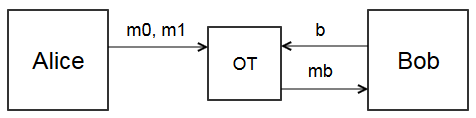
\includegraphics[scale=.8]{images/ot}
    \caption{The high level idea of oblivious transfer. Image from \cite{alexirpan}}
    \label{fig:basic-ot}
\end{figure}
Oblivious Transfer (OT) is a simple, useful protocol that underlies many more complicated crypto-systems \cite{EGL82, Rab05}.

Figure \ref{fig:basic-ot} outlines the high level idea of oblivious transfer.
The box in figure \ref{fig:basic-ot} may be thought of as a trusted post office.
Alice potentially sends two messages $m_0$ and $m_1$ to Bob, but instead of sending the messages to Bob, she sends the messages to the post office.
Bob, without seeing either $m_0$ or $m_1$, knows that he wants $m_b$ where $b \in \{0,1\}$, so he notifies the post office that he wants message $b$.
With this information, the post office gives Bob $m_b$.
We want two secure properties to hold: (1) Alice does not know whether Bob received $m_0$ or $m_1$ and (2) Bob does not learn any information about $m_{1-b}$, the message that he did not receive.

We will not focus on the internal operations of oblivious transfer; for our purposes, it is a secure black box.
When we use oblivious transfer in the next chapter, the two messages that Alice potentially sends will be encryption keys, and Bob will select a key that corresponds to his input - a value that he doesn't want Alice to know.
In Chapter 3 we discuss improvements to oblivious transfer, since oblivious transfer, despite its simple appearance, is computationally expensive.
%!TEX root = thesis.tex
\chapter{Classic 2PC}
\al{this paragraph is a little weak}
Secure Computation (SC) was first proposed in an oral presesntation by Andrew Yao \cite{yao-original}.
Since Yao's presentation, multiple methods for performing SC were developed.
One method was developed by Yao himself and is called garbled circuit.
Another was developed by a group of researchers, Goldreich, Micali and Widgerson \al{cite}.
The two methods are premised on a similar idea: encrypt a circuit by encrypting its gates, which has since been termed garbled circuit.
At this point, it is unclear which method is better, so researchers continue to study both methods.
\al{get source}

This chapter explains the two most prominent methods of SC for the two party case, referred to as Two-Party Protocol (2PC).
The first part of the chapter will motivate and describe desirable properties of a 2PC protocol, culminating in a definition. 
The second part of the chapter will describe in Yao's Garbled Circuits, a method for performing 2PC, and discuss security of 2PC.
The third part will provide an overview of GMW's method.

\section{2PC Security Motivation}
Think back to Alice and Bob from the introduction. 
Alice and Bob are millionaires who wish to determine who is wealthier without disclosing how much wealth they have.
More formally, Alice has input $x$ and Bob has input $y$ ($x$ and $y$ are integers corresponding to the wealth of each party), and they wish to compute the less than function $f$, such that 
\begin{equation}
f(x,y) = \left\{
\begin{array}{lr}
    1 & \text{if } x < y \text{;} \\
    0 & \text{otherwise.}
\end{array}
\right.
\end{equation} 

We call the overarching interaction between Alice and Bob protocol $\Pi$, and $\Pi$ consists of all messages exchanged and computations performed.
Based on the setup of the problem, we can list a few properties that Alice and Bob wish $\Pi$ to have.
\begin{description}
    \item[Privacy] 
        Parties only learn their output. 
        Any information learned by a single party during the execution of $\Pi$ must be deduced from the output. 
        For example, if Alice learns that she had more money after computing $f$, then she learns that $y < x$; however, this information about $y$ is deducible from the output therefore it is reasonable.
        It would be unreasonable if Alice learns that $1,000,000 < y < 2,000,000$, as that information is not deducible from $f(x,y)$.
    \item[Correctness] 
        Each party receives the correct output.
        In the case of Alice and Bob, this simply means that they learn correctly who has more money.
        In particular, correctness means that Alice and Bob \textit{both} learn the output.

\end{description}

One possible method for constructing a definition of security would be to list a number of properties a secure protocol must have.
This approach is unsatisfactory for a number of reasons.

One reason is that an import security property that is only relevant in certain cases may be missed.
There are many applications of 2PC, and in some cases, there may be certain properties that critical to security.
Ideally, a good definition of 2PC works for all applications, hence capturing all desirable properties.
A second reason that the property based definition is unsatisfactory is that the definition should be simple.
If the definition is simple, then it should be clear that \textit{all} possible attacks against the protocol are prevented by the definition.
A definition based on properties in this respect as it becomes the burden of the prover of security to show that all relevant properties are covered \cite{lindell2009secure}.

We must also think about the aims of each party involved in the protocol. 
Can we trust that parties are going to obey the protocol? 
It's relevant in the two party case, but if there are more than three parties, parties may either act independently or collude. 
These considerations are called the \textit{security setting}.
There are two primary security settings: the semi-honest setting and the malicious setting. 
The work presented in this thesis uses the semi-honest setting. 
In the semi-honest setting, we assume that each party obeys the protocol but tries to learn as much as possible from the information they are given.
This means that parties do not lie about their information, they do not abort, they do not send or withhold messages out of order, or deviate in any way from what is specified in the protocol. 
In contrast, the malicious setting considers that each party is liable to lie and cheat; parties can take any action to learn more information.

The malicious setting is much more realistic. 
Parties that are involved in cryptographic protocols are liable to lie and cheat, for why else would they even be engaged in the cryptographic protocol in the first place?
There are two main reasons why the semi-honest setting is useful.
The first is that many protocols can be constructed for the semi-honest setting, and then improved to function in the malicious setting.
There is a strong history of this occurring with protocols.
It's simply easier to think through and create protocols for the semi-honest setting; at the very least, it's a valuable starting point for building complex cryptosystems.
In the case of 2PC, there exist malicious protocols, and in fact, the primary 2PC protocol that this thesis uses, garbled circuits, can be improved to be malicious secure without too much difficulty. 

The second reason that the semi-honest setting is that it does have use cases in the real world.
There are some scenarios where parties want to compute a function amongst themselves, and trust each other to act semi-honestly.
One example is hospitals sharing medical data.
Hospitals are legally, and arguably ethically, restricted from sharing medical data, but this data can have great value especially when aggregated with datasets from other hospitals.
2PC offers hospitals the means to ``share'' their data, perform statistics and other operations on it, while keeping the data entirely private. 
Other examples where semi-honesty is sufficient include mutually trusting companies and government agencies.

\section{2PC Security Definition}
% http://crypto.stackexchange.com/questions/3814/simulation-based-security
% page 620 of Goldreich volume 2
In this section we discuss at a high level the definition of 2PC security, and then give the formal definition. 
The definition of security for 2PC protocols is the most complicated cryptographic theory that we have encountered thus far. 

Recall our setup: Alice and Bob are semi-honest parties with inputs $x$ and $y$ respectively who wish to compute the function $f: \{0,1\}^n \times \{0,1\}^n \to \{0,1\}^m \times \{0,1\}^m$.
Informally, we say $\Pi$ is scure if when $\Pi$ is executed in the real world, each party learns the same information as if they had completed the protocol in an ideal world.
The ideal world is where there is a trustred third party Carlo who receives the inputs $x$ from Alice and $y$ from Bob, computes the $f(x,y)$, and sends the output to Alice and Bob.
Carlo is honest and trusted, so we don't mind that he knows the inputs, and he is trusted to not share the inputs with the opposoring party.
This is the ideal world: the function is compute correctly, and no information about the inputs is shared to other parties.

In the real world, Alice and Bob do not have luxury of enlisting Carlo to perform their computation for them; instead, they use the 2PC protocol $\Pi$. 
To be confident that $\Pi$ is secure, we show that $\Pi$ in the real world is \textit{essentially the same} as Alice, Bob and Carlo acting in the ideal world.
Specifically, Alice and Bob should not learn any more information in the real world than they do in the ideal world.
If they do learn more information, then somewhere the protocol $\Pi$ is leaking information that cannot be deduced from the output of $f$. 
We show that the ideal is world is essentially the same as the ideal world by using the concept of computational indistinguishability presented in chapter 1.
To use computational indistinguishability, we need to build probability distrubtions of the information deducible in the real and ideal world.
Next, we construct probability distributions of the information that Alice and Bob can deduce from the ideal and real world.

To construct the probability distribution of the ideal world, we introduce \textit{simulators} $S_A$ and $S_B$.
$S_A$ and $S_B$ are probabilistic polynomial-time algorithms who are essentially adversaries, like the adversary in the definition of encryption from chapter 1, that specifically attack the ideal world.
Simulator $S_A$ takes as input $x$, Alice's input, and $f(x,y)$, the output of the function because that is the information that Alice has access to in the ideal world.
Likewise, $S_B$ takes input $y$ and $f(x,y)$, since that the is information that Bob has access to in the ideal world.

Given a simulator $S_A$, think about what the simulator can do.
The distribution of the its possible outputs is given by $\{S_A(x, f(x,y)\}_{x \in \{0,1\}^*}$.
Let us break this distribution down: $S_A$ is a fixed single algorithm.
$x$ is Alice's input, and $f(x,y)$ is the output of the function.
The set is indexed by all possible $x$, so all possible inputs that Alice could have.
In summary, $\{S_A(x, f(x,y)\}_{x \in \{0,1\}^*}$ represents the possible information that an algorithm could deduced from all possible $x$ and $f(x,y)$.
We think of $\{S_B(y, f(x,y)\}_{y \in \{0,1\}^*}$ for Bob's input similarly.

For constructing the probability distributions of the real world, we need to consider what information Alice and Bob have at their disposal.
Recall that Alice and Bob are semi-honest, which means that Alice and Bob follow all instruction of $\Pi$ correctly but they also will use any information they receive along the way.
More precisely, Alice and Bob obey the protocol, but also maintain a record of all intermediate computations.
We call Alice's record of intermediate computations Alice's \textit{view}, $\viewrv_A(x, y)$, which depends on inputs $x$ and $y$
And now we create the probability distribution for Alice: $\{\viewrv_A(x, y)\}_{x, y \in \{0,1\}^*}\}$.
This distribution represents the Alice's information from the intermediate computation indexed over all possible inputs $x$ and $y$.
Likewise, we call Bob's record of intermediate computations Bob's view,  $\viewrv_B(x, y)$, and his probability distribution of intermediate computations is $\{\viewrv_B(x, y)\}_{x,y \in \{0,1\}^*}\}$

To wrap it up, if $\Pi$ in the real world is the same as the Alice, Bob and Carlo in the ideal world, then the simulator $S_A$ and $S_B$ should only be able to learn what can be learned from the intermediate computations. 
That is, the probability distributions $\{S_A(x, f(x,y)\}_{x \in \{0,1\}^*}$ and $\{\viewrv_A(x, y)\}_{x, y \in \{0,1\}^*}\}$ should be essentially the same, i.e., computationally indstinguishable.

With this intuition in mind, we give Goldreich's definition of 2PC security from his textbook \textit{Foundations of Cryptography Volume II}\cite{goldreich}.

\begin{definition}
Let $f = (f_1, f_2)$ be a probabilistic, polynomial time functionality where Alice and Bob compute $f_1, f_2: \{0,1\}^n \to \{0,1\}^m$ respectively.
Let $\Pi$ be a two party protocol for computing $f$. 
Define $\viewrv_i^{\Pi}(n,x,y)$ (for $i \in \{1,2\}$) as the view of the $i$th party on input $(x,y)$ and security parameter $n$.
$\viewrv_i^{\Pi}(n,x,y)$ equals the tuple $(1^n, x, r^i, m_1^i, \ldots, m_t^i)$, where $r^i$ is the contents of the $i$th party's internal random tape, and $m_j^i$ is the $j$th message that the $i$th party received.
Define $output^{\Pi}_i(n,x,y)$ as the output of the $i$th party on input $(x,y)$ and security parameter $n$.
Also denote $ \outputrv^{\Pi}(n,x,y) = (\outputrv^{\Pi}_1(n,x,y), \outputrv^{\Pi}_2(n,x,y)).$
Note that $\viewrv^{\Pi}_i$ and $\outputrv^{\Pi}_i$ are random variables whose probabilities are taken over the random tapes of the two parties. Also note that for two party computation.

We say that $\Pi$ securely computes $f$ in the presence of static\footnote{\al{TODO} Mention what static means} semi-honest adversaries if there exist probabilistic polynomial time algorithms $S_1$ and $S_2$ such that for all $x,y \in \{0,1\}^*$, where $|x| = |y|$, the following hold:
\begin{equation} 
    \label{eqn:secdef1}
    \{(S_1(x, f_1(x,y), f(x,y)))\}_{x,y} \equiv^C \{(\viewrv^{\Pi}_1(x,y), \outputrv^{\Pi}(x,y)) \}_{x,y} 
\end{equation}
\begin{equation} 
    \label{eqn:secdef2}
    \{(S_2(x, f_2(x,y), f(x,y)))\}_{x,y} \equiv^C \{(\viewrv^{\Pi}_2(x,y), \outputrv^{\Pi}(x,y)) \}_{x,y} 
\end{equation}
\end{definition}

The definition requires that $|x| = |y|$; however, this constraint can be overcome by padding the shorter input.

A definition of 2PC security with malicious parties is substantially more complex.
For more information on a malicious security definition, we refer the reader to \cite{lindell2009}.

\section{Yao's Garbled Circuit}
We now discuss a popular 2PC scheme called garbled circuits.
At a high level, garbled circuits work by having one party, Alice, design a circuit that computes $f$ and encrypt (garble) that circuit.
Alice sends the encrypted circuit to Bob, along with some values corresponding to her and Bob's inputs, and Bob decrypts the circuit, acquring the output of $f(x,y)$ at the end.

\begin{figure}[h]
    \label{fig:thefig}
\centering
\begin{circuitikz} \draw
(0,2) node[and port] (myand1) {}
(0,0) node[and port] (myand2) {}
(3,1) node[xor port] (myxor) {}
(myand1.in 1) node[left=.8cm](a) {$x_0$}
(myand1.in 2) node[left=.8cm](b) {$x_1$}
(myand2.in 1) node[left=.8cm](c) {$y_0$}
(myand2.in 2) node[left=.8cm](d) {$y_1$}
(myxor.out) node[right=.5cm](e) {$z_0$}
(myxor.out) node[right=.25cm](f) {}
(a) -| (myand1.in 1)
(b) -| (myand1.in 2)
(c) -| (myand2.in 1)
(d) -| (myand2.in 2)
(myand1.out) -| (myxor.in 1)
(myand2.out) -| (myxor.in 2)
(myxor.out) -| (f)
;\end{circuitikz}
\caption{A simple boolean circuit. \al{Draw gate and wire number notation in here}}
\end{figure}

\al{figure numbering is off}
We now walk through how Alice garbles the circuit.
She starts with a typical boolean circuit, like the one shown in figure \ref{fig:thefig} \al{add figure of basic circuit with gates labeled}. 
In figure \ref{fig:thefig} the gates are ordered from $0$ to $2$, in order from nearest to the inputs to farthest from the inputs.
Alice begins by garbling gate $G_0$, the gate nearest to the inputs\footnote{Multiple gates at some point could equidistant from the input. In these cases, the ordering of gates does not matter.}.

% http://tex.stackexchange.com/questions/55213/how-to-draw-a-boolean-circuit-diagram-in-circuitikz
% http://texdoc.net/texmf-dist/doc/latex/circuitikz/circuitikzmanual.pdf
% adapted from figure on page 40

% Wires
Alice assigns two wire labels to each wire associated with gate $G_0$ - this includes wires $W_0$, $W_1$ and $W_5$.
For each wire, the zeroith label represents $0$ denoted $W_i^0$ and the other label represents $1$ denoted $W_i^1$ for the $i$th wire.
\al{explain what each wi label represents}
A wire labels is a ciphertext, the output of the encryption algorithm\footnote{A common encryption algorithm used now is AES-128, so the wire labels are 128 bit strings.}.
Alice assigns the wire labels by randomly sampling from $\{0,1\}^{\lambda}$, where $\lambda$ is the size of the output of the encryption algorithm.

After assigning labels to $W_0^0$, $W_0^1$, $W_1^0$, $W_1^1$, $W_5^0$ and $W_5^1$, Alice creates a garbled table $T_{G_0}$ for $G_0$.
Gate $G_0$ is an AND gate, and the structure of the table resembles the logical table for an AND gate.
The table has four columns. 
The first two columns are the input wire labels.
The third column is the wire labels for the output wire.
The wire label placed in the third column is based on logical operation of the AND gate.
For example, the third column and third row has the wire label associated with $0$, since AND outputs zero on input of $0$ and $1$.
The fourth column is the dual-key cipher encryption\footnote{See section \al{what section?} for information on dual-key ciphers} of the value in the third column, using the values of the first two columns as keys.
The garbled table for $G_0$ is shown in table \ref{tbl:g0-table}

\begin{table}[h]
\centering
\label{tbl:g0-table}
\begin{tabular}{|c|c|c|c|}
\hline
$W_0$ & $W_1$ & $W_5$ & Encryption \\
\hline
$W_0^0$ & $W_1^0$ & $W_5^0$ & $\Enc_{W_0^0, W_1^0}(W_5^0)$ \\
$W_0^1$ & $W_1^0$ & $W_5^0$ & $\Enc_{W_0^1, W_1^0}(W_5^0)$ \\
$W_0^0$ & $W_1^1$ & $W_5^0$ & $\Enc_{W_0^0, W_1^1}(W_5^0)$ \\
$W_0^1$ & $W_1^1$ & $W_5^1$ & $\Enc_{W_0^1, W_1^1}(W_5^1)$ \\
\hline
\end{tabular}
\caption{A garbled table for an AND gate with input wires $W_0$ and $W_1$ and output wire $W_5$.}
\end{table}

Alice creates wire labels for all remaining wires, and creates garbled tables all remaining gates.
She then sends the fourth column all of garbled tables to Bob.
The fourth column is an encryption of the gate.
Say a gate was input wires $W_i$ and $W_j$ and output wire $W_k$.
Bob can acquire a wire label of $W_k$ (i.e. $W_k^0$ or $W_k^1$) if he has one wire label of $W_i$ (i.e. $W_i^0$ or $W_i^1$) and one wire label of $W_j$ (i.e. $W_j^0$ or $W_j^1$).

Recall that Alice's input to the 2PC protocl are $x = x_0x_1$ where $x_1, x_0 \in \{0,1\}$.
Alice, to send her input to Bob, sends Bob the wire labels $W_0^{x_0}$ and $W_1^{x_1}$.
Bob does not know the values of $x_0$ or $x_1$, because he is simply receiving two ciphertexts, and does not know which value the ciphertexts represent.
The only information that Bob has is the fourth column of the garbled tables, and that does not provide any information about the sematic value of the wire labels.

Recall that Bob's input to the 2PC protocol is $y = y_0 y_1$ where $y_1, y_0 \in \{0,1\}$.
Alice now wants to send Bob $W_2^{y_0}$ and $W_3^{y_1}$, but does not know $y_0$ and $y_1$.
Alice and Bob can achieve this by using Oblivious Transfer, as described in chapter 1.
We focus on wire $W_2$.
Alice has two possible values that she wants to send to Bob: $W_2^0$ and $W_2^1$.
Alice only wants Bob to acquire one of the values, becuase otherwise he can decrypt multiple rows garbled table.
\al{introduce htis OT notation in chapter 1}
Bob wants to receive $W_2^{y_0}$, as that wire label corresponds to his input.
So Alice and Bob do $\OT(\{W_2^0, W_2^1\}, y_0)$, so that Alice obvliously sends Bob the correct wire label.
Alice and Bob also perform OT on wire $W_3$; in particular, they do $\OT(\{W_3^0, W_3^1\}, y_1)$.

Alice is finished garbling the circuit, and communicating information to Bob. 
Bob has everything he needs to ungarble, or decrypt, the circuit.
Bob starts with gate $G_0$, for which he has the fourth column of $T_{G_0}$, a wire label for wire $0$, which I denote $W_0^*$ since Bob does not which wire label it is, and $W_1^*$ accordingly.
Bob starts with the first row of $T_{G_0}$ and tries decrypting the value using $W_0^*$ and $W_1^*$.
Formally, Bob tries $\Dec_{W_0^*, W_1^*}(T_{G_0}\big[0\big])$ where $T_{G_0}\big[0\big]$ represents the value in the zeroith row of $T_{G_0}$.
Bob tries decrypting the values in all four rows of the garbled table $T_{G_0}$, but only one should work, since the other decryptions using the incorrect keys.
For Bob to recognize that encryption is failing, we add an additional property to the encryption scheme: the output of the decryption function should indicate whether the decryption was valid.
A single additional bit, where $0$ represents that decryption failed and $1$ represents that decryption was successful. 
It is noteworth that such a property is common to encrypion schemes, and can be added to any existing encryption if necessary.
With this property, as Bob tries decrtyping all four rows of the garbled table, only one should decrypt correctly.
Because of the way Alice constructed the garbled table, Bob knows that this correclty decrypted value is one of the wire labels of $W_5$, the output wire of gate $G_0$.
Bob then assigns this decrypted value to $W_5^*$, and uses the value as the input wire when decrypting gate $G_2$.

Bob repeats this same process for gate $G_1$ and for gate $G_2$.
For gate $G_2$, Bob uses wire labels $W_5^*$ and $W_6^*$ which he acquired by ungarbling gates $G_0$ and $G_1$.
Bob notifes Alice after acquiring $W_7^*$.
Alice sends him values $W_7^0$ and $W_7^1$.
If $W_7^* = W_7^0$, then the function output $0$ and Bob notifes Alice that the output was $0$.
Otherwise if $W_7^* = W_7^0$, then the function output $1$ and Bob notifes Alice that the output was $1$.

Bob and Alice have now securely computed the function.

\al{Match notation in this description with the algorithms}

\begin{algorithm}
\caption{Garble Circuit}
\label{alg:garble}
\begin{algorithmic}
    \Require Circuit $f(x,\cdot)$ 
    \Ensure Populate garbled tables $f(x,\cdot).tables$.
\For{wire $w_i$ in $f(x,\cdot).wires$} 
    \State Generate two encryption keys, called garbled values, $W_i^0$ and $W_i^1$.
    \State Assign $(W_i^0, W_i^1)$ to $w_i$.
\EndFor \\

\For{gate $g$ in $f(x,\cdot).gates$}
    \State Let $w_i$ be $g$'s first input wire.
    \State Let $w_j$ be $g$'s second input wire.
    \State Let $w_k$ be $g$'s output wire.
    \For{$(u,v) \in \{(0,0), (0,1), (1,0), (1,1)\}$}
    \State $T_g[u,v] = \Enc_{W_i^u}( \Enc_{W_j^v} ( W_k^{g(u,v)}))$
    \al{use DKC}
    \EndFor
    \State $f(x,\cdot).tables[g] = T_g$.
\EndFor
\end{algorithmic}
\end{algorithm}

\begin{algorithm}
\caption{Evaluate Circuit}
\label{alg:evaluate}
\begin{algorithmic}

\Require $(input\_wires, tables, gates)$
\For{Input wire $w_i$ in $input\_wires$}
	\Comment retrieve garbled values of input wires
	\State Perform OT$(w_i, x_i)$ 
	\Comment retrieve $W^{x_i}_i$ from Alice
	\State Save the value to $w_i$.
\EndFor

\For{Gate $g$ in $gates$}
	\Comment compute the output of each gate.
	\State Let $w_i$ be $g$'s first input wire.
	\State Let $w_j$ be $g$'s second input wire.
	\State Let $w_k$ be $g$'s output wire.
	\State \textbf{Require} $w_i$ and $w_j$ have been assigned garbled values.
	\State \textbf{Require} $w_k$ has not been assigned a garbled value.
    	\For{$(u,v) \in \{(0,0), (0,1), (1,0), (1,1)\}$}
        \al{use DKC}
		\State $temp = \Dec_{w_j}(\Dec_{w_i}(tables[g][u,v]))$
		\If{$temp$ decrypted correctly}
			\State $w_k = temp$
		\EndIf
	\EndFor
\EndFor
\end{algorithmic}
\end{algorithm}

\subsection{Step 0: Setup}
Alice and Bob wish to compute the function $f$, which is represented by a circuit (see section \ref{secn:circuit}).
Alice is the garbler, and will create and encrypt the circuit.
Bob is the evaluator, and will compute the circuit.

\subsection{Step 1: Garbling the Circuit}
\al{define a wire and a label}
Alice garbles each gate, according to algorithm \ref{lag:garble}, resulting in a table $T_g$ for each gate $g$.
The table enables the computation of a single gate $g$, if one is given either $W^0_i$ or $W^1_i$ and either $W^0_j$ or $W^1_j$ where wire $i$ and $j$ are the input wires to $g$.
Figure \ref{example} gives an example of a table for an AND gate.
\al{TODO}

\subsection{Step 2: Bob's Input and Computing the Circuit}
Alice sends the garbled circuit to Bob. 
The garbled circuit consists of a garbled table for each gate, $f(x,\cdot).tables$, and the rules for connecting the gates together.
In order for Bob to compute the circuit, he needs the garbled values of all input wires.
Once he has the garbled values of the input wires, he can decrypt the first few gates, and acquire the decryption keys of the other gates until he has the keys to decrypt all of the gates in the circuit, yielding the output.
Bob can acquire the garbled values of the input wires from Alice using 1-out-of-2 oblivious transfer on each input wire (see section \ref{sctn:oblivious_transfer}).
If necessary, Bob sends the final output of the circuit to Alice. 
This is necessary only if $f_1(x,y) = f_2(x,y)$. 
Bob's protocol is outlined in more detail in Algorithm \ref{alg:evaluate}.

\subsection{Explanation of the security of Yao's protocol}
To do.

\subsection{Notes about complexity}
1 OT per (input?) wire.
4 cts per gate.
How much encryption?
Not good enough for practice.

\section{GMW}
Where Yao's protocol is premised on encrypting gates individually, GMW's protocol for garbling circuits is premised on secret sharing, and performing operations on the shared secrets. 
Secret sharing, in general, is a class of methods for distributing a secret to a group of participants, where each participants is allocated a \textit{share} of the secret. 
The secret can only be reconstructed when a sufficient number of the participants combine their shares, but any pool of insufficient shares yields no information about the secret.

GMW begins by having Alice and Bob secret share their inputs, so each party now has a collection of \textit{shares}. 
Algorithm \ref{alg:gmw_setup} describes this process in more detail.
Then Alice and Bob perform a series of operations on their shares, which are dictated by the gates in the function they wish to compute.
As with Yao's protocol, a gate may either compute XOR, AND or NOT.
Each operation requires a different series of operations, which are described in Algorithm \ref{alg:gmw_gates}.
Finally, Alice and Bob publicize their shares to each other, at which point each party will have sufficient shares to compute the output of the function.

\begin{algorithm}[h!]
\caption{GMW Setup}
\label{alg:gmw_setup}
\begin{algorithmic}
% http://crypto.biu.ac.il/gmw-multi-party-protocol-and-oblivious-transfer-extension
    \State Alice does the following on input Circuit $f(x,\cdot)$ and $x = x_0x_1\ldots x_n$
    \For{wire $w_i$ in $f(x, \cdot).wires$}
        \State Assign $a^1_{w_i} \leftarrow \{0,1\}$
        \Comment a uniform random selection of $0$ or $1$.
        \State Assign $b^1_{w_i} = x_i \oplus a_{w_i}^1$
    \EndFor
    \State Bob does likewise on input Circuit $f(x,\cdot)$ and $y = y_0y_1\ldots y_n$
    \State Hence Alice has generated shares $\{a^1_w, b^1_w\}_w$ 
    \State and Bob has generated shares $\{a^2_w, b^2_w\}_w$
    \State Alice and Bob divide the shares such that Alice has all $a_w$ and Bob has all $b_w$.
\end{algorithmic}
\end{algorithm}

\begin{algorithm}
\caption{GMW Gate Evaluation}
\label{alg:gmw_gates}
\begin{algorithmic}
    \State \textbf{XOR Gate}
    \Comment $x_i \oplus y_i = (a_{w_i}^1 \oplus b_{w_i}^1) \oplus (a_{w_i}^2 \oplus a_{w_i}^2)$
    \State Alice evaluates $a_{w_i}^1 \oplus a_{w_i}^2$
    \State Bob evaluates $b_{w_i}^1 \oplus b_{w_i}^2$
    \\
    
    \State \textbf{AND Gate}
    \Comment $x_i \wedge y_i = (a_{w_i}^1 \oplus b_{w_i}^1) \wedge (a_{w_i}^2 \oplus a_{w_i}^2)$
    \State Alice samples $\sigma \leftarrow \{0,1\}$
    \Comment a uniform random selection of $0$ or $1$
    \State Alice constructs table $T$:
     \For{$(u,v) \in \{(0,0), (0,1), (1,0), (1,1)\}$}
     	\State $T[u,v] = (a^1_{w_i} \oplus u) \wedge (a^2_{w_i} \oplus v)$
	\State $s[u,v] = \sigma \oplus T[u,v]$.
     \EndFor    
     \State Do 1-4OT. Alice sends $(s[0,0], s[0,1], s[1,0], s[1,1])$ 
     \State Bob selects result based on $(u,v) = (b^1_{w_i}, b^2_{w_i})$.
    \\
    
    \State \textbf{NOT Gate}
    \Comment $w_i = (\neg a_{w_i}) \oplus (\neg b_{w_i})$
    \State $\triangleright$ Evaluate the negative of a particular wire $w_i$. 
    \State $w_i = a_{w_i} \oplus b_{w_i}$
    \State Let $a'_{w_i} = 1 \oplus a_{w_i}$
    \Comment i.e. $a'_{w_i} = \neg a_{w_i}$
    \State Let $b'_{w_i} = 1 \oplus b_{w_i}$
    \Comment i.e. $b'_{w_i} = \neg b_{w_i}$
\end{algorithmic}
\end{algorithm}

\al{see mike rosulek first few slides for good images. }
\al{illustration about translating bits over to wire labels}

\chapter{Improving MPC}
A number of improvements have been made to Yao's garbled circuit since its inception in 1986.
The first scheme for a garbled circuit, the one described in section \ref{garbled_circuit_scheme} has the following requirements: \textbf{include chart here}.
Let's look into how much work is required in classical garbled circuits.
\textbf{mention that we look gate-wise}
The first metric that we look at is the size of the garbled table.
\textbf{check this definition}:The garbled table, if you call recall from earlier, is the set of ciphertexts that is sent from the garbler to the evaluator, like in figure \ref{the fig thats a garbled table}.
Hence the size refers to the number of ciphertexts that an evaulator needs to compute a single gate.
The XOR column gives the size of the garbled table for an xor gate, and naturaly the AND columns gives the of the garbled table for an AND gate.
The cost associated with the size of a garbled table manifests in effecting the amount of bandwidth that needs to be transmitted between the garbler and evaluator.
In order to evaluate the gate, the evaluator needs the entire garbled table (\textbf{research idea: what if they don't? what if they can know when to request more information, to reduce the average amount of bandwidth? maybe this could be used to reduce calls to OT?)}, so reducing the size of the garbled table reduces bandwidth.
It turns out that bandwidth contributes a large hit to the total time required to perform mpc with garlbed circuits, and as a result, many of the improvements to garbled circuits have specifically targted reducing the size of the garbled table down from 4 ciphertexts.
\textbf{maybe mention lower bound?}

The second metric we use to analyze garbled circuits is eval cost.
Eval cost is the amount of computation that the evaluator must perform in order to process a single gate.
In the classical setting, the evaluator goes down the garbled table decrypting each ciphertext until one of the decrypts correctly. 
In the worst case, this requires 8 decryptions, because each wire is encrypted twice, once with the key from the first input wire and then again with the key from second input wire.
If a dual-key cipher (an encryption scheme that takes two keys, see section \ref{dkc section}), then the evaluator only needs to perform four decryptions in the worst case.
The metric that we consider is the garble cost of a gate. 
The garble cost of a gate is amount of computation that the garbler needs to perform.
The improvements to MPC have generally increased the garble cost; having the garbler do more work, can reduce the size of the garble table which reduces bandwidth, and can reduce the amount of computation the evaluator needs to perform \textbf{fact check this}.
Before the research of \cite{our_paper} and the research presented in this thesis, there were not substantial benefits to garbler preprocessing, that is having the garbler do work \textit{before} the actual computation time. 
We call this having the garbler do offline work, because they can do the work at their leisure, like at night when computers are less used.
Then the online work, when the actual comptuation is performed, is reduced.

As we walk through the improvements to Yao's garbled circuit, we are going to think about the improvements affect the three metrics described above.
It should also be noted before we begin that these are improvements to the the computation of a single gate.
Speedups on the gate level propagately widely through the computation of the entire garbled circuit.
For example, the computation of AES now requires approximatley $40,000$ gates, so reducing the number of ciphertexts being transmitted per gate by $1$, reduces the total amount of ciphertexts that need to be sent by $10,000$ - a substantial speedup indeed.

%\section{Overview of history}
%\begin{itemize}
%    \item working on specific function verse general functions
%    \item working on number of parties
%    \item making it work for sugarbeet auction
%    \item election potential?
%    \item auctions
%    \item ----- Mike talk -----
%    \item Things to think about:
%    \item hardness assumption (Mike does not focus on)
%    \item size: CTs/ per gate
%    \item computation required
%    \item Mike at 9:00 has cites to papers of big improvements
%    \item Focus is on improving each individual gate
%\end{itemize}

\section{Point and Permute}
Beaver, Micali and Rogaway contributed the first major improvement to Yao's garbled circuit in 1990.
A detail that I may or may not (\textbf{check this}) have left out in the description of Yao's garbled circuit is that the order of the garbled table needs to be permuted.
If the first key sent is always the key corresponding to the input wires's $0$ keys, then the evaluator can learn what the value of the input wires is - a violation of security.
The solution to this problem is easy: permute the order of the garbled table.
Now the evaulator trial decrypts each of the $4$ ciphertexts until there is a valid decryption .
\footnote{There exists encryption/decryption schemes that in addition to decrypting a ciphertext will also output a bit indicating if the decryption occurred correctly. Using schemes like this, the evaluator can decrypt all $4$ ciphertexts until one of them decrypts correctly, as indicated by the extra bit output by the decryption algorithm.}

The \textit{point and permute} technique speeds up the evaluator's computation of the garbled table by removing the need to trial decrypt the ciphertexts; instead, the garbler subtly communicates which single ciphertext to decrypt.
Using point and permute, the garbler randomly assigns a select bit $0$ or $1$ to each wire label in a wire \textbf{Is it clear what a wire label is, as opposed to a wire? Should be by now.}
The assignment of the select bit is independent of the truth value of the wire, so two things can happen. 
First, the garbler can permute the garbled table based on the select bits, and second, the select bits can be sent to the evaluator.
Upon receving the garbled table, the evaluator knows exactly which ciphertext to decrypt based on the select bits of the input wires.

Point and permute slightly increases the amoount of garbler-side computation to substantially decrease the amount of evaluator computation.
The garbler needs to sample $n+q$\footnote{Recall from \textbf{todo some previous section} that $n+q$ = number of wires.} additional random bits.
Without point and permute, the evaluator needs to decrypt $2.5$ ciphertexts on average, hence we estimate that there are roughly $1.5(n+q)$ fewer decryptions required.
The overall bandwidth is increased by $2$ bits per wire, from $256$ bits to $258$ bits: a small constant increase. \footnote{The value is constant in the sense that it is independent of the security parameter.}

\begin{table}[h]
    \centering
    \begin{tabular}{|c|c|}
    \hline
    Select Bit & Wire Label \\
    \hline
    0 & $A_0$ \\
    1 & $A_1$ \\
    1 & $B_0$ \\
    0 & $B_1$ \\
    \hline
    \end{tabular}
    \qquad
    \begin{tabular}{|c|c|}
    \hline
    Select Bits & Encryption \\
    \hline
    (0,0) & $\Enc_{A_0, B_1}(C_1)$ \\
    (0,1) & $\Enc_{A_0, B_0}(C_0)$ \\
    (1,0) & $\Enc_{A_1, B_1}(C_0)$ \\
    (1,1) & $\Enc_{A_1, B_0}(C_0)$ \\
    \hline
    \end{tabular}
    \qquad
    \begin{tabular}{|c|}
    \hline
    $C_0 \gets \{0,1\}^n$ \\
    $C_1 \gets \{0,1\}^n$ \\
    \hline
    \end{tabular}
    \caption{Garbled Gate for Point and Permute}
    \caption{Example garbled gate using point and permute. The gate being computed is given in figure \textbf{Make it 23:30 in mike's talk}}
\end{table}

\textbf{add chart if you want}

%\begin{itemize}
%    \item relative position of ciphertexts in table leaks information
%    \item so we have to permute the ciphertexts
%    \item when evaluating, trial decrypt all 4 until 1 works
%    \item beaver micali rogaway 90
%    \item randomly assign color (r,b) to each pair of wire label
%    \item Order the 4 cts canonically, by \emph{color} of keys: ((r,r),(r,b),(b,r),(b,b))
%    \item evaluate by decrypting ciphertexts indexed by your colors
%    \item Can use one-time-security encyption (e.g. OTP)
%    \item color independent of semantic value
%    \item show chart
%\end{itemize}

\section{Garbled Row Reduction 3}
Garbled Row Reduction 3 (GRR3) is technique proposed by \textbf{who} which decreases the number of ciphertexts that need be communicated between the garbler and evaluator.
To use GRR3, the garbler must also use the point and permute method.
Using Garbled Row Reduction, the garbler sets the ciphertext in the top row of the garbled table equal to a value that decrypts to $0^n$.
\footnote{In previous constructions the value for the ciphertext was chosen randomly.}
Upon evaluating the garbled gate, if the evaluator sees that the select bits of the input wires indicate to decrypt the first row, the evaluator simply assumes the ciphertext be of value $O^n$. 

\begin{table}[h]
    \centering
    \begin{tabular}{|c|c|}
    \hline
    Select Bit & Wire Label \\
    \hline
    0 & $A_0$ \\
    1 & $A_1$ \\
    1 & $B_0$ \\
    0 & $B_1$ \\
    \hline
    \end{tabular}
    \qquad
    \begin{tabular}{|c|c|}
    \hline
    Select Bits & Encryption \\
    \hline
    (0,1) & $\Enc_{A_0, B_0}(C_0)$ \\
    (1,0) & $\Enc_{A_1, B_1}(C_0)$ \\
    (1,1) & $\Enc_{A_1, B_0}(C_0)$ \\
    \hline
    \end{tabular}
    \qquad
    \begin{tabular}{|c|}
    \hline
    $C_0 \gets \{0,1\}^n$ \\
    $C_1 \gets \Enc_{A_0, B_1}^{-1}(0^n)$ \\
    \hline
    \end{tabular}
    \caption{Example garbled gate using point and permute and garbled row reduction 3. The gate being computed is given in figure \textbf{Make it 23:30 in mike's talk}}
\end{table}

Discuss security.

GRR3 does not have a significant effect on garbler side compuation.
The difference being that for constructing some wire lables, the garbler may need to compute $\Enc^{-1}$ instead of generating random bits. 
The evaluator needs to perform slightly less computation: in the event that the first row needs to be decrypted, the evaluator doesn't need to perform the decryption algorithm. 
This events occur with probabilty $\frac{1}{4}$, so we can extrapolate that the evaluator needs to perform $\frac{1}{4}$ fewer decryptions than wwould be necessary if only PP were being used.
GRR3 reduces the size of the garbled table from $4$ ciphertexts to $3$ ciphertexts, a $25\%$ reduction.

\section{Free XOR}
The Free XOR technique was developed by \textbf{who} in \textbf{when}.
The technique, as the name suggests, makes the computation of XOR gates essentially free.
Say the garbler is determining the lables for wire $A$.
The label associated with truth value $0$, $A_0$, is randomly sampled from $\{0,1\}^n$. 
Then the label assocated with the truth value is set such that $A_1 \gets A_0 \oplus \Delta$, where $\Delta$ is global, randomly sampled value from $\{0,1\}^n$.
If the garbler is garbling an XOR gate, then they set $C_0$ to $A \oplus B$, and like wire $A$, the garbler sets $C_1 = C_0 \oplus \Delta$.
With these wire labels, it turns out that the garbler doesn't need to send a garbled table: the evaluator can compute $C_0$ and $C_1$ by XORing the inputted wire labels.
The math for this operation is shown below:
\begin{align*}
    A \oplus B & = C \\
    (A \oplus \Delta) \oplus B & = (A \oplus B) \oplus \Delta = C \oplus \Delta \\
    A \oplus (B \oplus \Delta) & = (A \oplus B) \oplus \Delta = C \oplus \Delta \\
    (A \oplus \Delta) \oplus (B \oplus \Delta) & = (A \oplus B) \oplus (\Delta \oplus  \Delta) = C 
\end{align*}

\begin{table}[h]
    \centering
    \begin{tabular}{|c|c|}
    \hline
    Wire Label & Value\\
    \hline
    $A_0$ & $A$ \\
    $A_1$ & $A \oplus \Delta$ \\
    $B_0$ & $B$ \\
    $B_1$ & $B \oplus \Delta$ \\
    $C_0$ & $A \oplus B$ \\
    $C_1$ & $C_0 \oplus \Delta$ \\
    \hline
    \end{tabular}
    \qquad
    \begin{tabular}{|c|}
    \hline
    \hline
    \end{tabular}
    \caption{Example XOR garbled gate wires using PP, GRR3 and Free XOR.}
\end{table}

The Free XOR technique is also compatible with GRR3, but since XOR doesn't require a garbled table, GRR3 is only used on AND gates.

Using the Free XOR technique, the size of the garbled table is zero for all XOR gates and of size $3$ for AND gates.
This fact incentivizes the construction of circuits that optimize the number of XOR gates, minimize the number AND gates (while minimizing the size of the entire circuit of course).
One interesting implication of using the Free XOR technique is that an added assumption must be made to our encryption algorithm.
Since $\Delta$ is part of the key and part of the the payload\footnote{The payload is the value that is being encrypted} of the encryption algorithm, the encryption algorithm must be secure under the circularity assumption.
Fortunately, modern encryption uses AES-128, which is presumed to be secure under the circularity assumption.

%\begin{itemize}
%    \item post Fairplay
%    \item KolesnikovSchneider
%    \item $A,A \oplus \Delta$.
%    \item Note same delta every gate
%    \item Choose $C = A \oplus B$
%    \item XOR is then free: walk through that computatoin
%    \item Still works with GRR3
%    \item Because $\Delta$ is in the key and in the payload, requires circularity assumption
%    \item Incentivizes gates with as many xors as possible (has been done with AES -- why it's so fast)
%    \item Evaluator must konw what type of gate is being exectued: we have been assuming all along that the evaluator and garbler know the function.
%\end{itemize}

\section{Garbled Row Reduction 2}
Garbled row reduction 2 (GRR2) reduces the size of the garbled table for AND gates to $2$ ciphertexts, but it is not compatible with Free XOR, so XOR gates also require two ciphertexts.
The approach of GRR2 is quite different from GRR2. 
At a high level, it creates two third degree polynomials, one based on the input wires which should output $C_0$, and a second polynomial which should output $C_1$.
Since the polynomials are of three degrees, they are each uniquely generated by $3$ points. 
To construct the polynomials, the garbler uses $x,y,z$ for the first polynomail and $u,v,w$ for the second polynomial.
The garbler sends $x,y,u,v$ to the evaluator, who can interpolate the polynomial and plug in values $a,b,c$.

GRR2 is incompatible with Free XOR because the ciphertext values cannot be set to the xor of the inputer wires (e.g. $C \gets A \oplus B$), since the value of $C$ is always determined by the polynomial.

\textbf{Add to this, but no need to spend too much time on it since it's not used}

%\begin{itemize}
%    \item use unique deg-2 polynomial
%    \item use 2 second degree polynomials
%    \item then interpolate
%    \item can't do free xor.
%    \item because we have lost control of $C_0$ and $C_1$ (they are dependent on the polynomial)
%\end{itemize}

\section{FleXOR}
Before the creation of FlexXOR, MPC was at an awkward point where some circuits with a large amount of xors could be computed faster with Free XOR and circuits with fewer XORS could be computed faster with GRR2.
FleXOR serves as a method to reconcile GRR2 with Free XOR, solving the problem where the ciphertext values of AND gates are independent of $\Delta$.

FleXOR's construction is straightforward: use GRR2 on AND gates, and use Free XOR on XOR gates, correcting the delta value where necessary.
To correct the delta value, FleXOR adds in a unary gate that maps $A, A \oplus \Delta_1 \to A', A' \oplus \Delta_2$.

Suppose we have the following situation: we computing an XOR gate with input wires $A,B$ and output wire $C$.
Input wires $A$ and $B$ have each come from a different AND gate, so their labels are the result of the polynomial interpolation of GRR2.
To perform Free XOR, $A,B$ and $C$ need to be using the same delta value. 
The garbler adds an extra gate between $A$ and $B$ and the $XOR$ gate that adjusts their XOR value to the correct value.
The unary\footnote{Unary means has one input and one output.} gate maps $A,A \oplus \Delta_1 \to A', A' \oplus \Delta_2$, where $\Delta_2$ is the correct delta value for the XOR gate.

A garbled AND table costs $2$ ciphertexts, and a garbled XOR table costs $0,1$ or $2$ ciphertexts depending on how many ciphertexts need to be corrected.
This turns the creation of the circuit into a combinatorial optimization problem, where the offset of each wire needs to be determined to minimize the total cost of each XOR gate and be subject to the compatibility of GRR2 for AND gates.
Without doing too much (if any) optimization of the circuit, FleXOR usually requires $0$ or $1$ ciphertext in practice.

%\begin{itemize}
%    \item switch delta value: $A,A \oplus \Delta_1 \to A', A' \oplus \Delta_2$
%    \item cost a single ciphertext (after using GRR3 trick)
%    \item total cost 0,1,2 dependent on how many distinct deltas
%    \item make wire label outputs of AND gates based on polynomial interpolation (GRR2)
%    \item So we can do both free xor (which cost 0 CTs) and GRR2 (which cost 2 CTs per And gate + delta correction)
%    \item turns into combinatorial optimization problem: determine offset for each wire to minimize total cost of each xor gate + subject to compatibility of 2-CT row-reduction of AND gates.
%    \item in practice, seemed to usually require 0 or 1
%    \item still has circularity problem because based on free zor
%\end{itemize}

\section{Half Gates}
Half Gates is the most recent improvement Yao's garbled circuit.
The goal of Half Gates is to make AND gates cost two ciphertexts, while preserving properties necessary for Free XOR. 
I'm going to introduce Half Gates in a different way from the original paper.

We consider the case of an AND gate $c = a \wedge b$, where the generator knows the value of $a$. 
If $a = 0$, then the generator will create a unary gate that always outpost false, $c$. 
Otherwise if $a = 1$, then the generator create a unary identity gate that always outputs $b$. 
Table \ref{tbl:halfgate-gg-garb} shows the garbled gates for different values of $a$. 

%\begin{align*}
%& \text{If $a = 0$, then } 0 \wedge b = 0 \text{, so output } H(B) \oplus C. \\
%& \text{If $a = 1$, then } 1 \wedge b = b \text{, so output } H(B \oplus \Delta) \oplus C \oplus a\Delta .
%\end{align*}
\begin{table}[h]
    \label{tbl:halfgate-gg-garb}
    \centering
    \begin{tabular}{|c|}
    \hline
    Garbled Table for $a = 0$ \\
    \hline
    $H(B) \oplus C$ \\
    $H(B) \oplus C$ \\
    \hline
    \end{tabular}
    \begin{tabular}{|c|}
    \hline
    Garbled Table for $a = 1$ \\
    \hline
    $H(B) \oplus C$ \\
    $H(B) \oplus C \oplus \Delta$ \\
    \hline
    \end{tabular} $\;\rightarrow$
     \begin{tabular}{|c|}
    \hline
    Garbled Table for any $a$ \\
    \hline
    $H(B) \oplus C$ \\
    $H(B) \oplus C \oplus a\Delta$ \\
    \hline
    \end{tabular}
    \caption{Generator's Garbled Half Gate for $a = 0$, $a = 1$, and written more succinctly with $a\Delta$ for $a \in \{0,1\}$. If $a = 0$, then $a\Delta = 0$.  Otherwise if $a = 1$, then $a\Delta = \Delta$.}
\end{table}

Since the evaluator has the wire label corresponding to b (either $B$ or $B \oplus \Delta$), the evaluator can compute the label of the output wire of the AND gate by xoring the rows in the garbled table by $H(B)$ or $H(B \oplus \Delta)$ to get $C$ or $C \oplus \Delta$ respectively. 

A further improvement can be garnered by using the garbled row-reduction trick.
We choose $C$ such that the first of the top row of the garbled table is the all zeros ciphertext. 
The top row may not necessarily be $H(B) \oplus C$, since for security the rows are permuted. 
Because the top row is all 0s, it does not need to be sent to the evaluator. 
If the evaluator should decrypt the cipher text on the top row (as directed by point and permute), then the evaluator assumes the cipher text to be all 0s. Overall, computing $a \wedge b = c$ requires two having operations by the generator, a single hash operation by the evaluator, and the communication of one ciphertext. 

We now consider computing $a \wedge b = c$, where the evaluator somehow already knows the value of $a$.
If $a = 0$, then the evaluator should acquire $C$. 
Otherwise if $a = 1$, then the evaluator should acquire $C \oplus b\Delta$, in which case it is sufficient for the evaluator to obtain $\Omega = C \oplus B$ (then xor $\Omega$ with the wire label corresponding to $b$).
Table \ref{tbl:halfgate-gg-eval} shows cipher texts which the garbler gives to the evaluator.

This table is different from other garbled tables. 
First, the table does not need to be permuted. 
Secondly, evaluation is different.
If $a = 0$, then the evaluator uses wire label $A$ to decrypt the top row of the table and acquire $C$. 
If $a = 1$, then the evaluator uses $A \oplus \Delta$ to decrypt the second row, yielding $C \oplus B$.
The evaluator then xors wire label $B + b\Delta$ by $C \oplus B$ to obtain $C \oplus b\Delta$. 
As before, the ciphertext  on the top row does not need to be communicatd by using the garbled row-reduction trick.
The generator sets $C$ such that $H(A) \oplus C = 0$ (i.e. $C = H(A)$). 
The total cost of this half gate is the same as before: two hashes by the generator, one hash by the evaluator, and once cipher text. 

\begin{table}[h]
    \label{tbl:halfgate-gg-eval}
    \centering
    \begin{tabular}{|c|}
    \hline
    Garbled Table for any $A$ \\
    \hline
    $H(A) \oplus C$ \\
    $H(A \oplus \Delta) \oplus C \oplus B$ \\
    \hline
    \end{tabular}
    \caption{Evaluator's half gate garbled table.}
\end{table}

We now put the two half gates together to form an AND gate. 
Consider the following where $r$ is a random bit generated by the generator:
\begin{equation}
a \wedge b = a \wedge (r \oplus r \oplus b) = (a \wedge r) \oplus (a \wedge (r \oplus b)).
\end{equation}
The first AND gate, $a \wedge r$, can be computed with a generator-half-gate - the generator ``knows'' $r$. 
Furthermore, if we can let the evaluator know the value of $r \oplus b$, then the second AND gate, $(a \wedge (r \oplus b)$, can be computed with an evaluator-half-gate - the evaluator ``knows'' $r \oplus b$. 
And the final XOR can be computed with free xor at the cost of no ciphertexts. 

It is secure for the garbler to give $r \oplus b$ to the evaluator, since $r$ is random and blinds the value of $b$. 
The value of $r \oplus b$, while only a single bit, can be communicated to the evaluator for free: use the select bit (from the point and permute technique) of the false wire label on wire $b$ (so $r$ is the select bit on the true wire label of wire $b$).

The overall cost of using Half Gates for AND gates is four calls to $H$ for the generator, two calls to $H$ for the evaluator, and the communication of $2$ ciphertexts. 
Half Gates guarantees only two ciphertexts are needed per AND gate, but the tradeoff is the additional computation for both parties (i.e. computing $H$).
With FleXOR, the number of ciphertexts that need to be communicated may vary, but there is less computation required.

When MPC becomes used in real operations, the circuit will likely not be optimized for XOR gates (reducing the number of AND gates). 
In this case, where an arbitrary function is being computed, it is hypothesized that Half Gates will outperform FleXOR. 
But in many of the cases being examined now - most notably computing AES - the circuit has been optimized heavily to have very few AND gates, hence the benefits of Half Gates are less noticeable.\footnote{At present, the AES circuit is 80\% XOR gates} 

\begin{table}[h]
  \centering
  \renewcommand{\arraystretch}{1.2}
\begin{adjustbox}{width=1\textwidth}
  \begin{tabular}{|p{5cm}|c|c|c|c|c|c|c|}
    \hline
    \multirow{2}{5cm}{\centering \textbf{Garbled Circuit Improvement}} & 
    \multicolumn{2}{c|}{\textbf{Size (x$\lambda$)}} & 
    \multicolumn{2}{c|}{\textbf{Eval Cost}} & 
    \multicolumn{2}{c|}{\textbf{Garble Cost}} &
    \multirow{2}{3cm}{\centering \textbf{Assumption}} \\
    \cline{2-7}
    & \textbf{XOR} & \textbf{AND} & \textbf{XOR} & \textbf{AND}  & \textbf{XOR} & \textbf{AND} & \\
    \hline
    Classical & 1365 & 1260 & 1024 & $\mu$ s & a & b & a\\ \hline
    Point and Permute & TBD & TBD & TBD & $\mu$ s & a & b & a\\ \hline
    GRR3 & TBD & TBD & TBD & $\mu$ s  & a & b& a\\ \hline
    Free XOR & TBD & TBD & TBD & $\mu$ & a & bs& a  \\ \hline
    GRR2 XOR & TBD & TBD & TBD & $\mu$ & a & bs  & a\\ \hline
    FleXOR& TBD & TBD & TBD & $\mu$ & a & bs & a \\ \hline
    Half Gates & 2 & 0 & 2 & 0 & 4 & 0 & a \\ \hline
  \end{tabular}
  \end{adjustbox}
  \caption{Summary of Garbled Circuit Improvements. GRR3 stands for garbled row reduction 3 and GRR2 stands for garbled row reduction 2}
\end{table}

\section{Improving Oblivious Transfer}
\al{Fix this up}
Oblivious transfer has been improved in two relevant ways for 2PC protocols. 
These improvements are called OT-extension and OT-preprocessing. 
In OT-extension a constant number of OT's can be run to generate a polynomial number of exchanged values.
In OT-preprocessing the OT's occur before the actual protocol, during what is called the offline phase, and then when the OT's needed during the online phase, simpler and efficient communication realizes the exchanged values.
This is useful because the OT step requires a large amount of communication to be sent between the sender and receiver, often resulting in OT being the bottleneck of 2PC protocols.


\chapter{Chaining Garbled Circuits}

talk about our idea about chaining here.

%!TEX root = thesis.tex

\chapter{Implementation}

My largest contribution to the project of component-based garbled circuits is the implementation of the theoretical ideas in a program called \CompGC. 
The aim of \CompGC is to run a two party garbled circuit protocol from start to finish. 
The garbler and evaluator simply select a function to compute, plug their inputs into the system, and \CompGC securely computes the function.
This chapter describes the creation of \CompGC and presents experimental results. 

\section{\CompGC}

\CompGC was constructed over the period of 5 months in the programming language C. 
It consists of approximately $5,000$ lines of code, includes a submodule, \LibGarble, and includes python scripts to generate auxiliary files. 

\CompGC started with \JustGarble as its basic building block.
\JustGarble is a C-library written by Bellare et al. \cite{justgarble} that creates a garbled circuit given an inputted circuit, and evaluates the garbled circuit given input labels. 
It is a tool, supporting only garbling and evaluating operations, but does not perform the many operations needed for a whole secure system, like networking, oblivious transfer, and secure recovery of final outputs. 

I later replaced \JustGarble with \LibGarble, an improvement of \JustGarble, which was implemented by my colleague Alex Malozemoff.
\LibGarble made a number of improvements to \JustGarble, including cleaning up the API and improving the memory layout of  data-structures.
These improvements contributed to a substantial increase in performance: evaluating AES uses 17 cycles per gate in \LibGarble versus 22 cycles per gate in \JustGarble, a 22\% improvement. 
\LibGarble also adds the newest cryptographic technique, half-gates; However, \CompGC does not use half-gates since half-gates reduces the size of the garbled table at the cost of a single call to the hash function during evaluation. 
In the component-based garbled circuit setting, the garbled tables are communicated during offline time, and we are most concerned with online time when the hash function would be called; hence half-gates actually reduce performance.

\CompGC has an offline and an online phase. 
In the offline phase, \CompGC takes as input a list of circuits and creates a specified number of each circuit. 
The list of circuits could be small and focused, designed for computing a single function such as AES, or the list could be diverse, allowing for the computation of a variety of functions. 
\CompGC garbles the list of circuits the specified number of times, and then sends the garbled circuits with an attached identification number from the garbler to the evaluator. 
The garbler and evaluator each save the garbled circuits to disk. 
Finally, the garbler and evaluator perform the offline phase of preprocessed oblivious transfer. 
\CompGC uses the Naor-Pinkas semi-honest oblivious transfer protocol; the library for performing oblivious transfer was given to me by Alex Malozemoff \cite{naor-pinkas-ot}. 
The garbler finishes by saving the input labels and oblivious transfer data to disk, and similarly, the garbler saves the oblivious transfer data to disk. 
Algorithms \ref{alg:garbler-offline} and \ref{alg:evaluator-offline} show the steps taken by each party in the offline phase. 

In the online phase, the evaluator begins by loading the function to be computed from disk. 
We specify the function in a JSON format, in which the following information is laid out: components needed in the function, how components input and output wires are linked, where inputs should go, and what wires are outputs. 
We chose to use JSON because the file format is human readable, but a different format, such as a binary format, would be faster. 
As the functions become more complex, it becomes harder to write the function specification files. 
To overcome this, I wrote a python script that automatically generates the function specification file for various functions on arbitrary inputs. 

After the garbler loads the function specification file from disk, it generates a set of instructions for the evaluator. 
The instructions specify what components are used by naming them with the unique identification number assigned in the offline phase. 
The instructions further specify in what order to evaluate components, and how to link components. 
This step requires specifying the output wires of one garbled circuit, the input wires of another garbled circuit, and the linking value.
Finally, the instructions specify how to map the final output wire labels to bits; this works by sending unary gates, with a two-row garbled table, for each output wire. 

After the garbler sends the instructions to the evaluator, they both perform the online phase of oblivious transfer, whereby the evaluator acquires their input labels. 
The garbler next sends the input labels corresponding to their inputs. 
At this point, the evaluator has all the data they need to finish the protocol. 
They follow the instructions, and acquire the output bits. 
Algorithms \ref{alg:garbler-online} and \ref{alg:evaluator-online} summarize the online phase. 

\begin{algorithm}
    \caption{Garbler Offline}
    \label{alg:garbler-offline}
    \begin{algorithmic}
        \State \textbf{Input:} List of circuits, and number of ciphertexts to be OT-preprocessed.
        \State 1. Build circuits
        \State 2. Garble circuits (using \LibGarble)
        \State 3. Assign each garbled circuit an ID
        \State 4. Send garbled circuits and their IDs to evaluator
        \State 5. Save input labels and output labels of garbled circuit to disk
        \State 6. Perform offline phase of OT-preprocessing
        \State 7. Save data from OT-preprocessing to disk
    \end{algorithmic}
\end{algorithm}

\begin{algorithm}
    \caption{Evaluator Offline}
    \label{alg:evaluator-offline}
    \begin{algorithmic}
        \State 1. Receive garbled circuits from garbler
        \State 2. Save garbled circuits to disk
        \State 3. Perform offline phase of OT-preprocessing
        \State 4. Save OT-preprocessing data to disk
    \end{algorithmic}
\end{algorithm}

\begin{algorithm}
    \caption{Garbler Online}
    \label{alg:garbler-online}
    \begin{algorithmic}
        \State 1. Load input labels and output labels of garbled circuits from disk
        \State 2. Load OT-preprocessing data from disk
        \State 3. Load function specification from disk
        \State 4. Generate instructions from function specification
        \State 5. Compute chaining values, and add values to instructions
        \State 7. Perform online stage of OT-preprocessing
        \State 8. Send input wires correspond to garbler's input
        \State 9. Send instructions
    \end{algorithmic}
\end{algorithm}

\begin{algorithm}
    \caption{Evaluator Online}
    \label{alg:evaluator-online}
    \begin{algorithmic}
        \State 1. Load garbled circuits from disk
        \State 2. Load OT-preprocessing data from disk
        \State 3. Perform online stage of oblivious transfer - acquire evaluator's input labels
        \State 4. Receive garbler's input labels
        \State 5. Receive instructions
        \State 6. Following instructions, chaining and evaluating as instructed
    \end{algorithmic}
\end{algorithm}

\section{Experiments}
\CompGC experiments were run on an Intel Core i5-4210H CPU. 
They were conducted over two network settings. 
The first network setting ran both parties on the default localhost configuration, which was measured to have a latency of 0.012 ms and bandwidth of 25.2 Gb per second. 
The second network setting used the built in Linux network emulator {\sf netem} to configure localhost to mimic the latency and bandwidth of the internet. 
This included setting latency to 33 ms and bandwidth to 50 Mbits per second. 
Finally, \CompGC requires reading from disk; our experimental machine was measured to have cache reads speed of 6.7 GB per second and buffered disk reads speed of 96 MB per second.

We ran four experiments: AES, CBC mode, and Levenshtein distance with 30 symbols and with 60 symbols. 

In the AES experiment, we treated each round of AES as a separate component. AES has 10 rounds, and hence required linking 10 components. Moreover, we used 128-bit AES, meaning that each component link required linking 128 wires. 

CBC mode is an algorithm for encrypting messages of arbitrary length using a blockcipher, for which we used AES-128. 
We again used a single round of AES as a component, and we also used XOR component, which took 256 bits of input, and outputted their xor. 
For our experiment, we ran CBC mode on a 10 block message, a 1,280 bit string, thus requiring 110 components - 100 AES round components and 10 XOR components. 

Levenshtein distance is a measure of the difference between two strings which counts the minimum number of insertions, deletions or substitutions needed to transform one inputted string into the other inputted string. 
The most popular algorithm for computing Levenshtein distance is a dynamic program that runs in $\Theta(n^2)$. 
The algorithm is  two nested for loops where we run a procedure called \textit{Levenshtein-core} inside the inner for loop. 
Levenshtein-core takes five inputs - three distance values and two symbols - and it computes a new distance based on those five values.
For more information on the Levenshtein distance algorithm, we refer the reader to \cite{wiki-leven}. 

For our Levenshtein experiment, we use the Levenshtein-core circuit as a our only component; see figure \ref{fig:leven-core} for a description of the component.
If Levenshtein is being run on $n$-bit inputs, then we use $n^2$ Levenshtein-core components. 
Our experiment used an 8-bit alphabet and ran Levenshtein distance on strings of length 30 symbols and on strings of length 60 symbols, corresponding to 900 and 3600 components respectively. 

\begin{figure}
    \center
    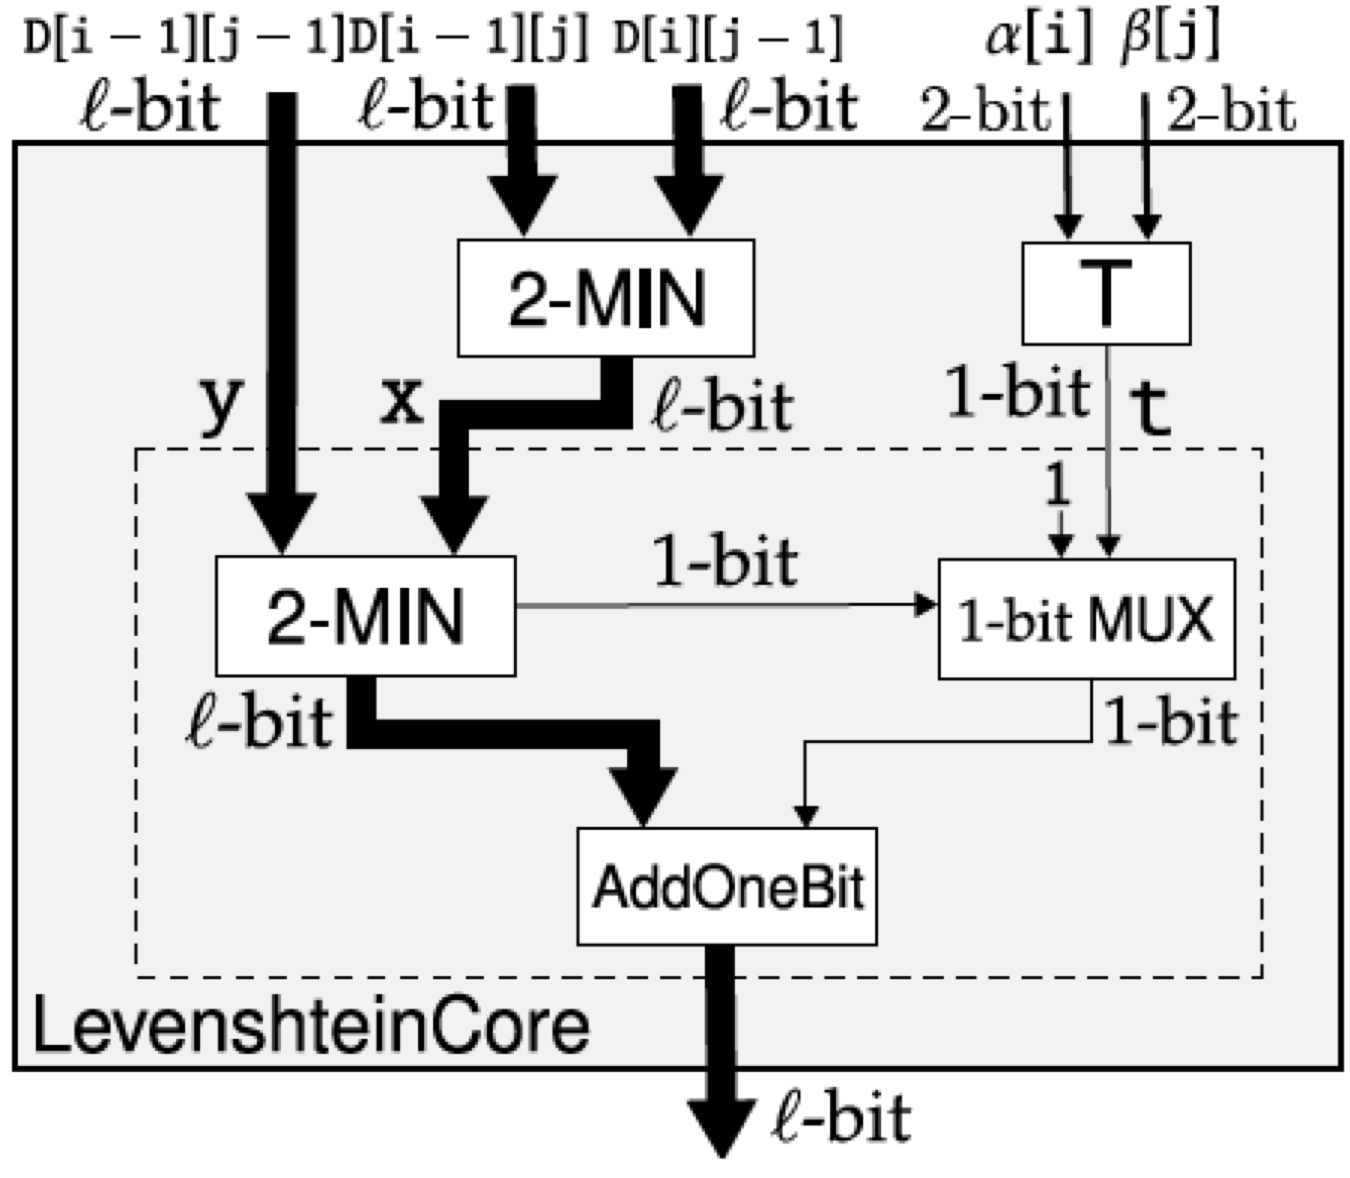
\includegraphics[scale=0.3]{images/leven_core}
    \caption[Levenshtein-core component]{The Levenshtein-core component used in the Levenshtein distance algorithm. 
    Levenshtein distance is a dynamic algorithm, and this is the only component used. 
    This particular version of Levenshtein-core was designed by \cite{faster2pc}.}
    \label{fig:leven-core}
\end{figure}

\section{Results}

\al{Should I say that I didn't run the experiments? That seems relevant.}

We ran experiments on the \CompGC system to compare component-based garbled circuits to standard 2PC garbled circuits, and to compare standard component-based garbled circuits to SCMC.

Table \ref{tbl:results} shows the online evaluator computation time, including time to load data from disk, of standard 2PC garbled circuits (implemented inside of the \CompGC system) and component-based garbled circuits with SCMC.
We give the average time of 100 trials and the 95\% confidence interval, the value after the $\pm$.
We see that larger circuits - Levenshtein 60 - offer more time savings than smaller circuits - AES; this is expected, since standard garbled circuits require that the entire circuit is communicated during online time, whereas the component-based garbled circuits sends the circuit during the offline phase. 

Table \ref{tbl:results-no-load} shows the same timing as table \ref{tbl:results} except we remove the time spent loading from disk.
Since \CompGC employs an offline phase, data is loaded from disk in the online phase. 
Table \ref{tbl:results-no-load} can be misleading - in what application do we assume that data is preloaded into RAM?
We include table \ref{tbl:results-no-load} because the literature often reports these times \cite{blazing-fast}. 
The times do have merit, as they highlight how CPU-bound the computation is, as opposed to measuring reading-from-disk speed, which can vary widely and is not something over which algorithm creators or programmers have much control. 

Table \ref{tbl:results-scmc} compares the speed of standard component based garbled circuits to SCMC.
We see approximately a 2x improvement for all of the experiments. 
However, these experiments do not highlight the benefit of SCMC. 
SCMC offers the greatest benefits in a large circuit where a large number of wires are used to represent a section of data.
Levenshtein distance, while a large circuit, has a small data-size: the data size of 60 symbol Levenshtein is only 6 bits. 
Consider circuits where an entire matrix is moved around between circuits; for example, linking a 10 by 10 matrix uses $800$ link labels if entries in the matrix were between $0$ and $256$, but SCMC uses a single link label.

\newpage
%!TEX root = thesis.tex
\begin{table}[h]

    %\tiny
    \scriptsize
    %\small
    %\footnotesize

    \centering
    \begin{tabular}{ r c c c c c c }
        &\multicolumn{2}{c}{\textbf{Time (localhost)}}
        &\multicolumn{2}{c}{\textbf{Time (simulated network)}}
        &\multicolumn{2}{c}{\textbf{Communication}} \\
        & \Naive & \CompGC & \Naive & \CompGC & \Naive & \CompGC  \\
        \midrule
        AES
        & 4.4 $\pm$ 0.0 ms
        & 3.0 $\pm$ 0.2 ms
        & 542.6 $\pm$ 0.7 ms
        & 68.5 $\pm$ 0.2 ms
        & 24 Mb & 254 Kb \\
        CBC, 10 blocks 
        & 45.8 $\pm$ 4.0 ms
        & 22.7 $\pm$ 1.4 ms
        & 4.8 $\pm$ 0.0 s
        & 216.7 $\pm$ 0.2 ms
        & 235 Mb & 2.6 Mb \\
        Leven, 30 symbols
        & 28.9 $\pm$ 6.6 ms
        & 24.3 $\pm$ 1.2 ms
        & 2.2 $\pm$ 0.0 s
        & 315.9 $\pm$ 0.5 ms
        & 108 Mb & 6.3 Mb \\
        Leven, 60 symbols
        & 109.8 $\pm$ 7.0 ms
        & 62.2 $\pm$ 0.7 ms
        & 10.6 $\pm$ 0.0 s
        & 742.5 $\pm$ 2.0 ms
        & 524 Mb & 25 Mb \\
    \end{tabular}
    \caption[Experimental results]{Experimental results.
        \Naive denotes standard semi-honest 2PC using garbled circuits and preprocessed OTs using \LibGarble,
        whereas \CompGC denotes our component-based implementation using SCMC. 
        Leven is Levenshtein distance.
        Time is online computation time, not including the time to preprocess OTs, but including the time to load data from disk.
        All timings are of the evaluator's running time, and are the average of 100 runs, with the value after the $\pm$ denoting the 95\% confidence interval.
        The communication reported is the number of bits received by the evaluator.
    }
    \label{tbl:results}
\end{table}

%!TEX root = thesis.tex

\begin{table}[h]
  \footnotesize
  \centering
  \begin{tabular}{ r c c c c }
    &\multicolumn{2}{c}{\textbf{Time (localhost)}}
    &\multicolumn{2}{c}{\textbf{Time (simulated network)}}\\
    & \Naive & \CompGC & \Naive & \CompGC \\
    \midrule
    AES
    & 4.4 $\pm$ 0.0 ms
    & 1.3 $\pm$ 0.1 ms
    & 542.6 $\pm$ 0.7 ms
             & 66.9 $\pm$ 0.1 ms \\
    CBC mode, 10 blocks
    & 45.8 $\pm$ 4.0 ms
    & 8.8  $\pm$ 0.5 ms
    & 4.8 $\pm$ 0.0 s
             & 204.3 $\pm$ 0.2 ms\\
    Levenshtein, 30 symbols
    & 28.9 $\pm$ 6.6 ms
    & 14.1 $\pm$ 0.4 ms
    & 2.2 $\pm$ 0.0 s
             & 305.6 $\pm$ 0.2 ms\\
    Levenshtein, 60 symbols
    & 109.8 $\pm$ 7.0 ms
    & 27.1 $\pm$ 0.4 ms
    & 10.6 $\pm$ 0.0 s
             & 703.4 $\pm$ 1.5 ms\\
  \end{tabular}
  \caption[Experimental results without loading time]{Experimental results without counting the evaluator time to load data from disk.}
  \label{tbl:results-no-load}
\end{table}

%!TEX root = thesis.tex

\begin{table}[h]
    \small
    \centering
    \begin{tabular}{ r c c c c }
        &\multicolumn{2}{c}{\textbf{Time (simulated network)}}
        &\multicolumn{2}{c}{\textbf{Communication}} \\
        & Standard & \scmc & Standard & \scmc \\
        \midrule
        AES
        & 134.4 $\pm$ 0.1 ms
        & 68.5 $\pm$ 0.2 ms
        & 656 Kb & 254 Kb \\
        CBC mode, 10 blocks 
        & 321.5 $\pm$ 0.9 ms
        & 216.7 $\pm$ 0.2 ms
        & 7.4 Mb & 2.6 Mb \\
        Levenshtein, 30 symbols
        & 371.0 $\pm$ 0.9 ms
        & 315.9 $\pm$ 0.5 ms
        & 10.0 Mb & 6.3 Mb \\
        Levenshtein, 60 symbols
        & 1119.6 $\pm$ 2.1 ms
        & 742.5 $\pm$ 2.0 ms
        & 44 Mb & 25 Mb \\
    \end{tabular}
    \caption[Comparison of naive protocol to SCMC]{Comparison of the two approaches for component-based garbled circuits: the standard approach and the \scmc approach.
    The experiments are run on the simulated network.}
    \label{tbl:results-scmc}
\end{table}

\newpage



\chapter{Experiments and Results}

talk about experiments and results here

\chapter{Future and Related Work}

talk about future and related work here

\chapter*{Conclusion}
         \addcontentsline{toc}{chapter}{Conclusion}
	\chaptermark{Conclusion}
	\markboth{Conclusion}{Conclusion}
	\setcounter{chapter}{4}
	\setcounter{section}{0}
	
Component-based garbled circuits offer a number of benefits in terms of flexiblity and speed over other garbled circuits methods.
This thesis contributes \CompGC, which demonstrates that component-based garbled circuit systems offer as much as as an order of magnitude improvements in terms of speed and bandwidth over other garbled circuit systems.

Chapter 1 of this thesis starts by explaining the cryptographic pritives necessary for understanding garbled circuits.
These primitives included encryption, oblivious transfer and the idea of computational indistinguishability.
In Chapter 2 we use the fundamentals introduced in Chapter 1 to discuss security of secure computation and garbled circuits.
We also introduce the basic garbled circuit protocol, and explain why it is secure under the earlier defition of security.
In Chapter 3 we discusses various improvements to garbled circuits, most of which operate by cleverly setting wire labels.
The most important improvement was Free XOR, which made XOR gates free, in the sense that they require no additional bandwidth.

In Chapter 4, we introduce component-based garbled circuits, a method of stitching together small component-circuits into a larger function.
We also discuss a contribution of this thesis to the literature: the idea of Single Commmunication Multiple Connections (SCMC).
SCMC reduces the bandwidth requirements of component-based garbled circuits by choosing input and output wire labels to have a predictable pattern.

Chapter 5 discusses \CompGC, our implementation of component-based garbled circuits.
\CompGC is a full-fledged two party secure computation system; parties select a function, select their inputs, and \CompGC runs a networked protocol between the two parties to compute the answer to their function.
We ran a number of experiments on \CompGC to test the improvements of SCMC over naive chaining, to compare component-based garbled circuits to traditional garbled circuits, and to examine the benefits of component-based garbled circuits in a real world networking setting by emulating the latency and bandwidth of the internet.
We found that \CompGC with SCMC is faster than all other garbled circuit protocols, and the speed is further emphasized when the systems are run on the emulated internet.
\CompGC reduced the online bandwidth of garbled circuits by approximatately, but this is for functions that are commonly tested in the literature.
Functions with larger pieces of data, such as stastical operations in the real world or large genomic analysis, are optimal for the component-based system.

Overall, we conclude that component-based garbled circuits improve garbled circuits by improving flexibility, speed and bandwidth of secure computation in the two party case.



\appendix
\chapter{The First Appendix}
\chapter{The Second Appendix, for Fun}


%This is where endnotes are supposed to go, if you have them.
%I have no idea how endnotes work with LaTeX.

\backmatter % backmatter makes the index and bibliography appear properly in the t.o.c...

% if you're using bibtex, the next line forces every entry in the bibtex file to be included
% in your bibliography, regardless of whether or not you've cited it in the thesis.
\nocite{*}

% Rename my bibliography to be called "Works Cited" and not "References" or ``Bibliography''
% \renewcommand{\bibname}{Works Cited}

% \bibliographystyle{bsts/mla-good} % there are a variety of styles available; 
% \bibliographystyle{plainnat}
% replace ``plainnat'' with the style of choice. You can refer to files in the bsts or APA 
% subfolder, e.g. 
%\bibliographystyle{acm}  % or
\bibliographystyle{APA/apa-good}  % or
\bibliography{thesis}
% Comment the above two lines and uncomment the next line to use biblatex-chicago.
%\printbibliography[heading=bibintoc]
% Finally, an index would go here... but it is also optional.
\end{document}
